\documentclass[12pt]{article}
\usepackage[spanish,es-tabla,es-nodecimaldot]{babel}
\usepackage{tikz}
\usepackage{amsmath}    %Caracteres especiales de matematicas
\usepackage[hidelinks]{hyperref}    % Vinculos [que no estén subrayados]
\usepackage{listings}   %Introducir codigo
\usepackage{setspace}
\usepackage{color}
\usepackage{amssymb}
\usepackage[makeroom]{cancel}
\usepackage{pdflscape}  %Voltear la página
\usepackage{tcolorbox}  %Cuadros de teoremas
\usepackage{fancyhdr, lastpage}
\usepgflibrary{fpu}
\usepackage{ifthen}
\usepackage{graphicx}
\usepackage{caption}
\usepackage{subcaption}
\usepackage{multirow}
\usepackage{tikz-3dplot}
\usepackage{pgfplots}
\usepgfplotslibrary{external}
\tcbuselibrary{listings,theorems}
\usepackage{wrapfig}
\usepackage{rotating}


\pagestyle{fancy}   %Encabezado en las páginas
\chead{Probabilidad, procesos aleatorios e inferencia}  %Encabezado central
\lhead{}    %Encabezado izquiero vacio
\rhead{}    %Encabezado derecho vacio
%% Cambiar letra a tamaño 12

\usepackage[Glenn]{fncychap}
% Sonny, Lenny, Glenn, Conny, Rejne, Bjarne, Bjornstrup

\providecommand{\abs}[1]{\lvert#1\rvert}

\definecolor{Code}{rgb}{0,0,0} 
\definecolor{Decorators}{rgb}{0.5,0.5,0.5} 
\definecolor{Numbers}{rgb}{0.5,0,0} 
\definecolor{MatchingBrackets}{rgb}{0.25,0.5,0.5} 
\definecolor{Keywords}{rgb}{0,0,1} 
\definecolor{self}{rgb}{0,0,0} 
\definecolor{Strings}{rgb}{0,0.63,0} 
\definecolor{Comments}{rgb}{0,0.63,1} 
\definecolor{Backquotes}{rgb}{0,0,0} 
\definecolor{Classname}{rgb}{0,0,0} 
\definecolor{FunctionName}{rgb}{0,0,0} 
\definecolor{Operators}{rgb}{0,0,0} 
\definecolor{Background}{rgb}{0.98,0.98,0.98} 


\lstset{frame=tb,
numbers=left, 
numberstyle=\footnotesize, 
numbersep=1em, 
xleftmargin=1em, 
framextopmargin=2em, 
framexbottommargin=2em, 
showspaces=false, 
showtabs=false, 
showstringspaces=false, 
frame=l, 
tabsize=4, 
% Basic 
basicstyle=\ttfamily\small\setstretch{1}, 
backgroundcolor=\color{Background}, 
% Comments 
commentstyle=\color{Comments}\slshape, 
% Strings 
stringstyle=\color{Strings}, 
morecomment=[s][\color{Strings}]{"""}{"""}, 
morecomment=[s][\color{Strings}]{'''}{'''}, 
% keywords 
morekeywords={import,from,class,def,for,while,if,is,in,elif,else,not,and,or,print,break,continue,return,True,False,None,access,as,,del,except,exec,finally,global,import,lambda,pass,print,raise,try,assert}, 
keywordstyle={\color{Keywords}\bfseries}, 
% additional keywords 
morekeywords={[2]@invariant,pylab,numpy,np,scipy}, 
keywordstyle={[2]\color{Decorators}\slshape}, 
emph={self}, 
emphstyle={\color{self}\slshape}, 
}


\newcommand{\tdplotmainfig}{%
%Angle Definitions
%-----------------
%
%set the plot display orientation
%synatax: \tdplotsetdisplay{\theta_d}{\phi_d}
\tdplotsetmaincoords{60}{110}
%
%define polar coordinates for some vector
%TODO: look into using 3d spherical coordinate system
\pgfmathsetmacro{\rvec}{.8}
\pgfmathsetmacro{\thetavec}{30}
\pgfmathsetmacro{\phivec}{60}
%
%start tikz picture, and use the tdplot_main_coords style to implement the display coordinate transformation provided by 3dplot
\begin{tikzpicture}[scale=3,tdplot_main_coords]

	%set up some coordinates 
	%-----------------------
	\coordinate (O) at (0,0,0);

	%determine a coordinate (P) using (r,\theta,\phi) coordinates.  This command also determines (Pxy), (Pxz), and (Pyz): the xy-, xz-, and yz-projections of the point (P).
	%synatax: \tdplotsetcoord{Coordinate name without parentheses}{r}{\theta}{\phi}
	\tdplotsetcoord{P}{\rvec}{\thetavec}{\phivec}

	%draw figure contents
	%--------------------

	%draw the main coordinate system axes
	\draw[thick,->] (0,0,0) -- (1,0,0) node[anchor=north east]{$x$};
	\draw[thick,->] (0,0,0) -- (0,1,0) node[anchor=north west]{$y$};
	\draw[thick,->] (0,0,0) -- (0,0,1) node[anchor=south]{$z$};

	%draw a vector from origin to point (P) 
	\draw[-stealth,color=red] (O) -- (P);

	%draw projection on xy plane, and a connecting line
	\draw[dashed, color=red] (O) -- (Pxy);
	\draw[dashed, color=red] (P) -- (Pxy);

	%draw the angle \phi, and label it
	%syntax: \tdplotdrawarc[coordinate frame, draw options]{center point}{r}{angle}{label options}{label}
	\tdplotdrawarc{(O)}{0.2}{0}{\phivec}{anchor=north}{$\phi$}


	%set the rotated coordinate system so the x'-y' plane lies within the "theta plane" of the main coordinate system
	%syntax: \tdplotsetthetaplanecoords{\phi}
	\tdplotsetthetaplanecoords{\phivec}

	%draw theta arc and label, using rotated coordinate system
	\tdplotdrawarc[tdplot_rotated_coords]{(0,0,0)}{0.5}{0}{\thetavec}{anchor=south west}{$\theta$}

	%draw some dashed arcs, demonstrating direct arc drawing
	\draw[dashed,tdplot_rotated_coords] (\rvec,0,0) arc (0:90:\rvec);
	\draw[dashed] (\rvec,0,0) arc (0:90:\rvec);

	%set the rotated coordinate definition within display using a translation coordinate and Euler angles in the "z(\alpha)y(\beta)z(\gamma)" euler rotation convention
	%syntax: \tdplotsetrotatedcoords{\alpha}{\beta}{\gamma}
	\tdplotsetrotatedcoords{\phivec}{\thetavec}{0}

	%translate the rotated coordinate system
	%syntax: \tdplotsetrotatedcoordsorigin{point}
	\tdplotsetrotatedcoordsorigin{(P)}

	%use the tdplot_rotated_coords style to work in the rotated, translated coordinate frame
	\draw[thick,tdplot_rotated_coords,->] (0,0,0) -- (.5,0,0) node[anchor=north west]{$x'$};
	\draw[thick,tdplot_rotated_coords,->] (0,0,0) -- (0,.5,0) node[anchor=west]{$y'$};
	\draw[thick,tdplot_rotated_coords,->] (0,0,0) -- (0,0,.5) node[anchor=south]{$z'$};

	%WARNING:  coordinates defined by the \coordinate command (eg. (O), (P), etc.) cannot be used in rotated coordinate frames.  Use only literal coordinates.  

	%draw some vector, and its projection, in the rotated coordinate frame
	\draw[-stealth,color=blue,tdplot_rotated_coords] (0,0,0) -- (.2,.2,.2);
	\draw[dashed,color=blue,tdplot_rotated_coords] (0,0,0) -- (.2,.2,0);
	\draw[dashed,color=blue,tdplot_rotated_coords] (.2,.2,0) -- (.2,.2,.2);

	%show its phi arc and label
	\tdplotdrawarc[tdplot_rotated_coords,color=blue]{(0,0,0)}{0.2}{0}{45}{anchor=north west,color=black}{$\phi'$}

	%change the rotated coordinate frame so that it lies in its theta plane.  Note that this overwrites the original rotated coordinate frame
	%syntax: \tdplotsetrotatedthetaplanecoords{\phi'}
	\tdplotsetrotatedthetaplanecoords{45}

	%draw theta arc and label
	\tdplotdrawarc[tdplot_rotated_coords,color=blue]{(0,0,0)}{0.2}{0}{55}{anchor=south west,color=black}{$\theta'$}

\end{tikzpicture}
}

\newcommand{\threedcoord}[2]{%
\tdplotsetmaincoords{#1}{#2}
\begin{tikzpicture}[tdplot_main_coords]
	\draw[thick,->] (0,0,0) -- (1,0,0) node[anchor=north east]{$x$};
	\draw[thick,->] (0,0,0) -- (0,1,0) node[anchor=north west]{$y$};
	\draw[thick,->] (0,0,0) -- (0,0,1) node[anchor=south]{$z$};
\end{tikzpicture}
}

\newcommand{\threedrotcoordsystem}{%
\tdplotsetmaincoords{50}{140}
\begin{tikzpicture}[scale=5,tdplot_main_coords]
	\draw[thick,->] (0,0,0) -- (1,0,0) node[anchor=north east]{$x$};
	\draw[thick,->] (0,0,0) -- (0,1,0) node[anchor=north west]{$y$};
	\draw[thick,->] (0,0,0) -- (0,0,1) node[anchor=south]{$z$};

	\tdplotsetrotatedcoords{34}{26}{12}

	\draw[thick,color=blue,tdplot_rotated_coords,->] (0,0,0) -- (.5,0,0) node[anchor=north east]{$x'$};
	\draw[thick,color=blue,tdplot_rotated_coords,->] (0,0,0) -- (0,.5,0) node[anchor=north west]{$y'$};
	\draw[thick,color=blue,tdplot_rotated_coords,->] (0,0,0) -- (0,0,.5) node[anchor=south]{$z'$};
	
\end{tikzpicture}
}

\newcommand{\threedconventions}{%
\tdplotsetmaincoords{50}{110}
\begin{tikzpicture}[scale=2,tdplot_main_coords]
	\draw[thick,->] (0,0,0) -- (1,0,0) node[anchor=north east]{$x$};
	\draw[thick,->] (0,0,0) -- (0,1,0) node[anchor=north west]{$y$};
	\draw[thick,->] (0,0,0) -- (0,0,1) node[anchor=south]{$z$};

	\draw[color=blue] (0,0,0) -- (.5,.5,0);

	\draw[color=blue,->] (.5,0,0) arc (0:45:.5);	
\end{tikzpicture}
}


\newcommand{\threedalphabetagamma}{%
\beginpgfgraphicnamed{Figures/alphabetagamma}
\tdplotsetmaincoords{50}{140}
%
\begin{tikzpicture}[scale=2,tdplot_main_coords]
	\draw[thick,->] (0,0,0) -- (1,0,0) node[anchor=north east]{$x$};
	\draw[thick,->] (0,0,0) -- (0,1,0) node[anchor=north west]{$y$};
	\draw[thick,->] (0,0,0) -- (0,0,1) node[anchor=south]{$z$};

	\tdplotsetrotatedcoords{0}{0}{30}

	\draw[thick,color=red,tdplot_rotated_coords,->] (0,0,0) -- (.7,0,0) node[anchor=north]{$x'$};
	\draw[thick,color=green!50!black,tdplot_rotated_coords,->] (0,0,0) -- (0,.7,0) node[anchor=west]{$y'$};
	\draw[thick,color=blue,tdplot_rotated_coords,->] (0,0,0) -- (0,0,.7) node[anchor=west]{$z'$};
	
	\tdplotdrawarc[color=orange!50!black]{(0,0,0)}{.4}{0}{30}{anchor=north east}{$\gamma$}
\end{tikzpicture}
%
\begin{tikzpicture}[scale=2,tdplot_main_coords]
	\draw[thick,->] (0,0,0) -- (1,0,0) node[anchor=north east]{$x$};
	\draw[thick,->] (0,0,0) -- (0,1,0) node[anchor=north west]{$y$};
	\draw[thick,->] (0,0,0) -- (0,0,1) node[anchor=south]{$z$};

	\tdplotsetrotatedcoords{0}{0}{30}

	\draw[dashed,color=red,tdplot_rotated_coords] (0,0,0) -- (.5,0,0);
	\draw[dashed,color=green!50!black,tdplot_rotated_coords] (0,0,0) -- (0,.5,0);
	\draw[dashed,color=blue,tdplot_rotated_coords] (0,0,0) -- (0,0,.5);

	\tdplotsetrotatedcoords{0}{40}{30}

	\draw[thick,color=red,tdplot_rotated_coords,->] (0,0,0) -- (.7,0,0) node[anchor=north]{$x'$};
	\draw[thick,color=green!50!black,tdplot_rotated_coords,->] (0,0,0) -- (0,.7,0) node[anchor=west]{$y'$};
	\draw[thick,color=blue,tdplot_rotated_coords,->] (0,0,0) -- (0,0,.7) node[anchor=south]{$z'$};
	
	\tdplotsetthetaplanecoords{0}
	\tdplotdrawarc[tdplot_rotated_coords,color=orange!50!black]{(0,0,0)}{.4}{0}{40}{anchor=south}{$\beta$}

\end{tikzpicture}
%
\begin{tikzpicture}[scale=2,tdplot_main_coords]
	\draw[thick,->] (0,0,0) -- (1,0,0) node[anchor=north east]{$x$};
	\draw[thick,->] (0,0,0) -- (0,1,0) node[anchor=north west]{$y$};
	\draw[thick,->] (0,0,0) -- (0,0,1) node[anchor=south]{$z$};

	\tdplotsetrotatedcoords{0}{40}{30}

	\draw[dashed,color=red,tdplot_rotated_coords] (0,0,0) -- (.5,0,0);
	\draw[dashed,color=green!50!black,tdplot_rotated_coords] (0,0,0) -- (0,.5,0);
	\draw[dashed,color=blue,tdplot_rotated_coords] (0,0,0) -- (0,0,.5);

	\tdplotsetrotatedcoords{60}{0}{0}
	\draw[dotted,color=blue,tdplot_rotated_coords] (0,0,0) -- (.4,0,0);
	\tdplotsetrotatedcoords{60}{40}{30}

	\draw[thick,color=red,tdplot_rotated_coords,->] (0,0,0) -- (.7,0,0) node[anchor=north]{$x'$};
	\draw[thick,color=green!50!black,tdplot_rotated_coords,->] (0,0,0) -- (0,.7,0) node[anchor=west]{$y'$};
	\draw[thick,color=blue,tdplot_rotated_coords,->] (0,0,0) -- (0,0,.7) node[anchor=south]{$z'$};


	\tdplotdrawarc[color=orange!50!black]{(0,0,0)}{.2}{0}{60}{anchor=north east}{$\alpha$}
\end{tikzpicture}
\endpgfgraphicnamed
}


\begin{document}
\title{Probabilidad, procesos aleatorios e inferencia}
\author{Ana Maritza Bello Ya\~nez}
\maketitle


%%%%%%%%%%%%%%%%%%%%%%%%%%%%%%%%%%%%%%%%%%%%%%%%%%%%%%%%%%%%%%%%%%%%%
%                       Caja del teorema                            %
%                                                                   %
\newtcbtheorem{theorem}{Teorema}             %
{colback=gray!5,colframe=gray!35!black,fonttitle=\bfseries}{th}   %
%%%%%%%%%%%%%%%%%%%%%%%%%%%%%%%%%%%%%%%%%%%%%%%%%%%%%%%%%%%%%%%%%%%%%

\tableofcontents

\setlength{\parindent}{0pt}
\setlength{\parskip}{0em}
\pagebreak
\section*{Resumen: La belleza y utilidad de las matem\'aticas}

Las matem\'aticas han impregnado todos los campos de la actividad cient\'ifica y
desempe\~nan un papel inestimable en la biolog\'ia, la f\'isica, la qu\'imica,
la econom\'ia, la sociolog\'ia y la ingenier\'ia.


El descubrimiento simult\'aneo ha ocurrido a menudo en la historia de las
matem\'aticas.

Por ejemplo el del c\'alculo del erudito ingl\'es Isaac Newton (1643-1727) y el
matem\'atico alem\'an Gottfried Wilhelm Leibniz (1646-1716). Esto nos hacen
preguntarnos por qu\'e se hicieron estos descubrimientos cient\'ificos en al
mismo tiempo por personas que trabajan de forma independiente. Para dar otro
ejemplo, los naturalistas brit\'anicos Charles Darwin (1809–1882) y Alfred
Wallace (1823–1913) desarrollaron la teor\'ia de la evoluci\'on de manera
independiente y simult\'anea. De manera similar, el matem\'atico h\'ungaro
J\'anos Bolyai (1802–1860) y el matem\'atico ruso Nikolai Lobachevsky
(1793–1856) parec\'ian haber desarrollado la geometr\'ia hiperb\'olica de forma
independiente y al mismo tiempo.

Lo m\'as probable es que tales descubrimientos simult\'aneos hayan ocurrido
porque el momento era propicio para tales descubrimientos, dado el conocimiento
acumulado por la humanidad en el momento en que se realizaron los
descubrimientos. A veces, dos cient\'ificos se sienten estimulados al leer la
misma investigaci\'on preliminar de uno de sus contempor\'aneos. Por otro lado,
los m\'isticos han sugerido que existe un significado m\'as profundo para tales
coincidencias.

En ocasiones, se han utilizado teor\'ias matem\'aticas para predecir fen\'omenos
que no se confirmaron hasta a\~nos despu\'es. Por ejemplo, las ecuaciones de
Maxwell, llamadas as\'i por el f\'isico James Clerk Maxwell, predijeron las
ondas de radio. Las ecuaciones de campo de Einstein sugirieron que la gravedad
doblar\'ia la luz y que el universo se est\'a expandiendo. El f\'isico Paul
Dirac se\~nal\'o una vez que las matem\'aticas abstractas que estudiamos ahora
nos dan una idea de la f\'isica en el futuro. De hecho, sus ecuaciones
predijeron la existencia de antimateria, que posteriormente fue descubierta. De
manera similar, el matem\'atico Nikolai Lobachevsky dijo que “no hay rama de las
matem\'aticas, por abstracta que sea, que alg\'un d\'ia no pueda aplicarse a los
fen\'omenos del mundo real”.



\section{Problemas del milenio}

\subsection{Problemas P vs NP}
Se trata del primero de los problemas del milenio de las matemáticas aplicadas,
y alude más concretamente al campo de la complejidad computacional, dentro del
ámbito de la informática. Su planteamiento se remonta a los años 70, cuando
además de por Alan Turing, fue planteado paralelamente por los programadores
Stephen Cook y Leonid Levin.

A grandes rasgos, el problema P frente a NP busca clasificar los problemas en
dos clases: los que pueden ser resueltos con una cantidad determinada de
recursos, y aquellos que no. Los recursos a los que nos referiríamos serían el
tiempo empleado para realizar los cálculos, y la memoria requerida (no olvidemos
que nos encontramos en el campo de la informática computacional) para procesar
los datos del problema.

Por ejemplo, los problemas P serían de fácil resolución para las computadoras, es
decir sus soluciones serían fáciles de encontrar en una cantidad razonable de
tiempo. En los problemas NP, por el contrario, la solución podría ser muy
difícil de encontrar, o quizá requeriría una gran cantidad de recursos (miles de
años), para ser hallada, aunque una vez encontrada la solución sería fácil de
comprobar. Un ejemplo muy ilustrativo de este tipo de problemas podría ser la
resolución de un puzle, donde encontrar el orden de las piezas, podría requerir
gran cantidad de recursos, pero una vez terminado el puzzle, la solución
correcta saltaría a la vista, y sería fácil de comprobar.

El problema P versus NP plantea si todos los problemas NP son también un
problema P. Si P es igual a NP, todos los problemas NP contendrían un atajo
oculto, que permitiría que los ordenadores encontrasen rápidamente soluciones
perfectas. Pero si P no es igual a NP, entonces no existen dichos atajos, lo que
demostraría que la potencia de resolución de problemas de los ordenadores es
limitada.

\subsection{Hipótesis de Riemann}

La hipótesis de Riemann fue formulada por primera vez por Bernhard Riemann en
1859, y por su relación con la distribución de los números primos en el conjunto
de los naturales, es uno de los problemas abiertos más importantes en la
matemática contemporánea. Riemann sugirió que la distribución de estos números
está estrechamente relacionada con el comportamiento de la llamada "función zeta
de Riemann", la cual tiene dos tipos de ceros: los ceros "triviales", que son
todos los números enteros pares y negativos; y los ceros "no triviales", cuya
parte real está siempre entre 0 y 1.

La hipótesis de Riemann afirma que todos los ceros no triviales de la función
zeta se encuentran en la recta $x = 1/2$. A día de hoy, más de diez billones de
ceros han sido calculados para la función $z$, todos alineados sobre la recta
crítica, los cuales corroboran la sospecha de Riemann. Sin embargo todavía nadie
aún ha podido demostrar en la actualidad que la función zeta no tenga ceros no
triviales fuera de dicha recta.

\subsection{La conjetura de Poincaré}

La conjetura de Poincaré es un problema topológico, establecido en 1904 por el
matemático francés Henri Poincaré. Se trataba de uno de los problemas de más
difícil resolución de los 7 problemas del milenio. Decimos "se trataba" por que
fue resuelto en el año 2006, convirtiéndose en el Teorema de Poincaré como fruto
del trabajo del matemático ruso Grigori Perelman, quien renunció a la cuantía
económica del premio.

El teorema sostiene que la esfera cuatridimensional, también llamada 3-esfera o
hiperesfera, es la única variedad compacta cuatridimensional en la que todo lazo
o círculo cerrado (1-esfera) se puede deformar (transformar) en un punto. Este
último enunciado es equivalente a decir que solo hay una variedad cerrada y
simplemente conexa de dimensión: la esfera cuatridimensional.




\section{Experimentos deterministas vs aleatorios}


\begin{tcolorbox}[colback=gray!5!white,colframe=gray!60!black,title=Definición: Observación]
    Cualquier registro de informaci\'on, ya sea num\'erico o categ\'orico.
\end{tcolorbox}

Ejemplos: 

Los n\'umeros 2, 0, 1 y 2, que representan el n\'umero de accidentes que
ocurrieron cada mes, de enero a abril, durante el a\~no pasado, constituyen un
conjunto de observaciones. 

Lo mismo ocurre con los datos categ\'oricos N, D, N, N y D, que representan los
art\'iculos defectuosos o no defectuosos cuando se inspeccionan cinco
art\'iculos y se registran como observaciones \cite{walpole2012probabilidad}.

\begin{tcolorbox}[colback=gray!5!white,colframe=gray!60!black,title=Definición: Experimento]
    Cualquier proceso que genere un conjunto de datos.    
\end{tcolorbox}

Un ejemplo simple de experimento estad\'istico es el lanzamiento de una moneda
al aire. En tal experimento s\'olo hay dos resultados posibles: águila o sol.
\cite{walpole2012probabilidad}.

\begin{tcolorbox}[colback=gray!5!white,colframe=gray!60!black,title=Definición: Tipos de experimentos]

    \textbf{Experimento determinista.}
    Un experimento determinista es aquel que produce el mismo resultado cuando se le
    repite bajo las mismas condiciones.

    \tcblower

    \textbf{Experimento aleatorio.}
    Un experimento aleatorio es aquel que, cuando se le repite bajo las mismas
    condiciones, el resultado que se observa no siempre es el mismo y tampoco es
    predecible.
\end{tcolorbox}



\section*{Teoría de conjuntos}

\subsection*{Introducción}

El concepto de conjunto, es fundamental en matemáticas. Su estudio, se basa en
el hecho de que éstos pueden ser combinados, mediante ciertas operaciones, para
formar otros conjuntos. 

El estudio de las operaciones con los conjuntos, constituye el álgebra de
conjuntos; que tiene semejanzas formales (aunque también presenta diferencias)
con el álgebra de los números. El álgebra de conjuntos, resulta valiosa en la
reducción de los conceptos matemáticos a sus fundamentos lógicos. 

La disciplina matemática que estudia las propiedades generales de los conjuntos
es la teoría de conjuntos. Esta disciplina se comenzó a desarrollar,
rigurosamente, a finales del siglo XIX y principios del XX. El fundador de dicha
teoría es el matemático alemán de origen ruso, George Ferdinand Ludwing
Phillipp Cantor (1845, 1918). Las ideas y conceptos de la teoría de conjuntos
han irrumpido literalmente en todas las ramas de las matemáticas y cambiaron su
faz por completo.

\subsection*{Definición básica de conjunto}

Un conjunto es cualquier colección de objetos bien definidos por medio de alguna
o algunas propiedades en común, de dichos objetos. Por objeto entenderemos no
sólo cosas físicas, como discos, computadores, etc., si no también abstractos,
como son números, letras, etc. A los objetos se les llama elementos del
conjunto.

Representamos a los conjuntos por medio de letras mayúsculas, así $A$, $B$, $C$,
etc., nos representan conjuntos.

\subsection*{Elemento}

Se llaman elementos o miembros a los objetos que componen un conjunto; y se
denotan con letras minúsculas, como: $a, b, x, y$, etc. Para indicar que un
objeto $x$ pertenece o es miembro de un conjunto $A$, escribimos $x \in A$, que
se lee \textit{“x elemento de A”} y, si no pertenece al conjunto $A$, escribimos
$x \notin A$, que se lee \textit{“x no es elemento de A”}.

\subsection*{Conjunto universo}
Llamamos conjunto universo y lo denotamos por $\mathbb U$, al conjunto del cual se
seleccionan los elementos para formar conjuntos.

En general identificamos al conjunto universo como un todo, pero no
representamos de una manera única a este “todo”, así habrá ocasiones que un
conjunto sea considerado conjunto universo y en otras no, por ejemplo:
considerando el conjunto P de los número pares, se tiene que

\begin{tabular}{ |l|l|l| }
    
\multirow{2}{4em}{$\mathbb C$ conjunto de los complejos} & \multirow{2}{4em}{$\mathbb R$ números reales} \\
    & & $\mathbb I$ números irracionales \\
    & & $\mathbb Q$ números racionales
    %& & {$\mathbb Z$ números enteros}
\end{tabular}



\subsection*{Conjunto vacío}

El conjunto vacío o nulo es un conjunto que no tiene elementos, el conjunto
vacío se representa por: $\emptyset$, o bien por \{\}.

No confundir el conjunto $A = \emptyset $ con el conjunto $ A = \{\emptyset\} $,
ya que el primer conjunto indica que no tiene ningún elemento y el segundo
conjunto indica que tiene un elemento y ese elemento es el conjunto vacío.

\subsection*{Igualdad de conjuntos}

Decimos que dos conjuntos $A$ y $B$ son iguales y denotamos $A=B$, si y solo si
$A$ es un subconjunto de $B$, y $B$ es un subconjunto de $A$.

\begin{equation}
    A=B \iff A \subseteq B \land B \subseteq A
\end{equation}

\subsection*{Subconjunto}

Si todos los elementos de un conjunto $A$ son también elementos de un conjunto
$B$, esto es, si cuando $x \in A$ entonces $x \in B$ (simbólicamente $x \in A
\rightarrow x \in B$), decimos que $A$ es un subconjunto de $B$ o que $A$ está
contenido en $B$ y se escribe:

\begin{equation}
    A \subseteq B \iff (\forall x)|[x \in A \rightarrow x \in B]
\end{equation}

Si $A$ no es subconjunto de $B$ se escribe $A \not \subseteq B$ .

Si además existe un elemento de $B$ que no este en $A$, decimos que $A$ es un
subconjunto propio de $B$ y se denota $A \subset B$ o $B \subset A$ y es
equivalente a la siguiente preoposición:

\begin{equation}
    (\exists \ x \in \mathbb U)[x \in A \land x \not\in B]
\end{equation}

\subsection*{Propiedades de los conjuntos}

\begin{enumerate}
    \item Si $A$ es cualquier conjunto diferente del vacío, entonces $A \subseteq A$ .
    Esto es, cualquier conjunto diferente del vacío es subconjunto de si mismo.

    \item El conjunto vacío es subconjunto de cualquier conjunto distinto del vacío,
    esto es $\emptyset \subset A$

    \item Si $n>0$ es el número de elementos de $A$ entonces el número de elementos
de $P(A)$ es $2^n$
\end{enumerate}

\begin{theorem}{Conjuntos}{conjuntos}
Sean $A$ y $B$ dos conjuntos. Decimos que $A=B$ si y solo si $A \subseteq B$ y
$B \subseteq A$
\end{theorem}

\begin{theorem}{Conjuntos}{conjuntos}
    Si $ A \subset B $ y $ B \subset C $, entonces $ A \subset C $
\end{theorem}

\subsection*{Cardinalidad}

Sea $A$ un conjunto, la cardinalidad de $A$ es el número de elementos diferentes
del conjunto $A$ y se representa por $|A|$.

\subsection*{Conjunto potencia}
Sea $A$ un conjunto finito, llamaremos conjunto potencia al conjunto formado por
todos los subconjuntos de $A$. El conjunto potencia se denota como $P(A)$ o bien
$2^A$.

\subsection*{Operaciones entre conjuntos}

% Definition of circles
\def\firstcircle{(0,0) circle (1.5cm)}
\def\secondcircle{(0:2cm) circle (1.5cm)}
\def\rectangle{(-2,-2) rectangle (4,2)}

\colorlet{circle edge}{blue!50}
\colorlet{circle area}{blue!20}

\tikzset{filled/.style={fill=circle area, draw=circle edge, thick},
    outline/.style={draw=circle edge, thick}}

\setlength{\parskip}{5mm}

\subsubsection*{Unión}

La unión de dos conjuntos $A$ y $B$, denotada por $ A \cup B $ (que se lee “A
unión B”) es un nuevo conjunto formado por los elementos que pertenecen a $A$ o
a $B$ o a ambos conjuntos.

\begin{equation}
    A \cup B = \{x | x \in A \vee x \in B\}
\end{equation}

Si $x \in A \cup B $ entonces $x \in A $ ó $x \in B$ o $x$ pertenece a ambos
conjuntos.

% Set A or B
\begin{figure}[h]
    \centering
    \begin{tikzpicture}
        \draw \rectangle;
        \draw[filled] \firstcircle node {$A$}
                      \secondcircle node {$B$};
        \node[anchor=south] at (current bounding box.north) {$A \cup B$};
    \end{tikzpicture}
    \caption{Representación gráfica de la unión de conjuntos $A \cup B$}
    \label{fig:unionConjuntos}
\end{figure}

\subsubsection*{Intersección}

La intersección de dos conjuntos $A$ y $B$, denotada por $A \cap B$ (que se lee
“ A intersección B”), es un nuevo conjunto formado por los elementos que
pertenecen a A y a B al mismo tiempo, es decir, por los elementos comunes a
ambos conjuntos.

\begin{equation}
    A \cap B=\{x | x \in A \wedge x \in B\}
\end{equation}

% Set A and B
\begin{figure}[h]
    \centering
    \begin{tikzpicture}
        \draw \rectangle;
        \begin{scope}
            \clip \firstcircle;
            \fill[filled] \secondcircle;
        \end{scope}
        \draw[outline] \firstcircle node {$A$};
        \draw[outline] \secondcircle node {$B$};
        \node[anchor=south] at (current bounding box.north) {$A \cap B$};
    \end{tikzpicture}
    \caption{Representación gráfica de la intersección de los conjuntos de $A \cap B$.}
    \label{fig:interseccionConjuntos}
\end{figure}

\subsubsection*{Complemento}

Sea $A \subseteq U$ un conjunto. El complemento de A denotado por $\bar{A}$,
$A'$, $A^C$ ó $U-A$, se define como el conjunto de todos los elementos que están
en $U$ pero no están en $A$. Simbólicamente:

\begin{equation}
    \bar{A}= \{x | x \in \mathbb U \wedge x \notin A\}
\end{equation}

Es decir, el complemento de $A$ es el conjunto de los todos los elementos que no
están en el conjunto $A$. Simbólicamente: $ \bar{A}={x | x \notin A}$.

% Set A^c
\begin{figure}[h]
    \centering
    \begin{tikzpicture}
        \draw[filled] \rectangle node [anchor=north west] at (current bounding box.north) {$\bar{A}$};
        \begin{scope}
            \clip \firstcircle;
            \fill[white!80] \firstcircle;
            \draw[draw=circle edge,thick] \firstcircle node {$A$};
        \end{scope}
        \node[anchor=south] at (current bounding box.north) {$\bar{A}$};
    \end{tikzpicture}
    \caption{Representación gráfica del complemento de $\bar{A}$}
    \label{fig:unionConjuntos}
\end{figure}

\subsubsection*{Diferencia}

Sean $A$ y $B$ dos conjuntos, definimos la diferencia de $A$ y $B$, que se
denota por $A-B$, como el conjunto de todos los elementos que pertenecen a $A$
pero no pertenecen a $B$. Simbólicamente:

\begin{equation}
    A-B = \{x | x \in A \land x \not\in B\}
\end{equation}

% Set A but not B
\begin{figure}[h]
    \centering
    \begin{subfigure}[b]{0.45\textwidth}
        \centering
        \begin{tikzpicture}
            \draw \rectangle;
            \begin{scope}
                \clip \firstcircle;
                \draw[filled, even odd rule] \firstcircle node {$A$}
                                             \secondcircle;
            \end{scope}
            \draw[outline] \firstcircle
                           \secondcircle node {$B$};
            \node[anchor=south] at (current bounding box.north) {$A - B$};
        \end{tikzpicture}
    \end{subfigure}
\hfill
    \begin{subfigure}[b]{0.45\textwidth}
        \centering
        % Set B but not A
        \begin{tikzpicture}
            \draw \rectangle;
            \begin{scope}
                \clip \secondcircle;
                \draw[filled, even odd rule] \firstcircle
                                             \secondcircle node {$B$};
            \end{scope}
            \draw[outline] \firstcircle node {$A$}
                           \secondcircle;
            \node[anchor=south] at (current bounding box.north) {$B - A$};
        \end{tikzpicture}
\end{subfigure}
\caption{Representación gráfica de la diferencia de los conjuntos de $A-B$ y de $B-A$.}
\label{fig:diferenciaConjuntos}
\end{figure}

\subsubsection*{Diferencia simétrica}
La diferencia simétrica de dos conjuntos $A$ y $B$, se denota como $A \triangle
B$, se define como la unión de $A-B$ y $B-A$. Simbólicamente:

\begin{equation}
    A \triangle B = (A-B) \cup (B-A)
\end{equation}


%Set A or B but not (A and B) also known a A xor B
\begin{figure}[h]
    \centering
    \begin{tikzpicture}
        \draw \rectangle;
        \draw[filled, even odd rule] \firstcircle node {$A$}
                                     \secondcircle node{$B$};
        \node[anchor=south] at (current bounding box.north) {$A \triangle B$};
    \end{tikzpicture}
    \caption{Representación gráfica de la diferencia simétrica de los conjuntos de $A \triangle B$.}
    \label{fig:diferenciaSimetricaConjuntos}
\end{figure}

\subsection*{Propiedades del álgebra de conjuntos}

\begin{itemize}

\item \textbf{Idempotencia}
\begin{equation}
    \begin{array}{ll}
        A \cup A & = A \\
        A \cap A & = A
    \end{array}
\end{equation}

\item \textbf{Conmutatividad}
\begin{equation}
    \begin{array}{ll}
        A \cup B & = B \cup A \\
        A \cap B & = A \cap B
    \end{array}
\end{equation}

\item \textbf{Asociatividad}
\begin{equation}
    \begin{array}{ll}
        (A \cup B) \cup C & = A \cup (B \cup C) \\
        (A \cap B) \cap C & = A \cap (B \cap C)
    \end{array}
\end{equation}

\item \textbf{Distributividad}
\begin{equation}
    \begin{array}{ll}
        A \cup (B \cap C) & = (A \cup B) \cap (A \cup B) \\
        A \cap (B \cup C) & = (A \cap B) \cup (A \cap B)
    \end{array}
\end{equation}

\item \textbf{Identidad}
\begin{equation}
    \begin{array}{ll}
        A \cup \emptyset & = A \\
        A \cap \mathbb{U} & = A
    \end{array}
\end{equation}

\item \textbf{Dominación}
\begin{equation}
    \begin{array}{ll}
        A \cap \emptyset & = A \\
        A \cup \mathbb{U} & = A
    \end{array}
\end{equation}

\item \textbf{Inversa}
\begin{equation}
    \begin{array}{ll}
        A \cup \bar{A} & = \mathbb U \\
        A \cap \bar{A} & = \emptyset
    \end{array}
\end{equation}

\item \textbf{Complemento}
\begin{equation}
    \begin{array}{ll}
        \bar{\bar{A}} & = A \\
        \bar{\mathbb U} & = \emptyset \\
        \bar{\emptyset} & = \mathbb U \\
    \end{array}
\end{equation}

\item \textbf{DeMorgan}
\begin{equation}
    \begin{array}{ll}
        \bar{A \cup B} & = \bar{A} \cap \bar{B} \\
        \bar{A \cap B} & = \bar{A} \cup \bar{B}
    \end{array}
\end{equation}

\item \textbf{Absorción}
\begin{equation}
    \begin{array}{ll}
        A \cup (A \cap B) & = A \\
        A \cap (A \cup B) & = A
    \end{array}
\end{equation}

\end{itemize}



\section{Binomio de Newton}

El binomio de Newton consiste en una fórmula que permite obtener los
coeficientes de un término enésimo de un binomio elevado a un exponente
determinado.

La fórmula matemática del binomio de Newton es la siguiente:

\begin{equation}
    (a+b)^n = \sum_{k=0}^{n} \binom{n}{k} a^{n-k} b^k
\end{equation}

\subsection{Desarrollo del binomio de Newton de la potencia 1 a la 10}

\begin{landscape}
	\begin{equation}
		\begin{split}
			(a+b)^0 &   = 1 \\
			(a+b)^1 &   = a+b \\
			(a+b)^2 &   = a^2+2ab+b^2 \\
			(a+b)^3 &   = a^3+3a^2b+3ab^2+b^3 \\
			(a+b)^4 &   = a^4+4a^3b+6a^2b^2+4ab^3+b^4 \\
			(a+b)^5 &   = a^5+5a^4b+10a^3b^2+10a^2b^3+5ab^4+b^5\\
			(a+b)^6 &   = a^6+6a^5b+15a^4b^2+20a^3b^3+15a^2b^4+6ab^5+b^6\\
			(a+b)^7 &   = a^7+7a^6b+21a^5b^2+35a^4b^3+35a^3b^4+21ba^2b^5+21ab^6+b^7 \\
			(a+b)^8 &   = a^8+8a^7b+28a^6b^2+56a^5b^3+70a^4b^4+56a^3b^5+28a^2b^6+8ab^7+b^8 \\
			(a+b)^9 &   = a^9+9a^8b+36a^7b^2+84a^6b^3+126a^5b^4+126a^4b^5+84a^3b^6+36a^2b^7+9ab^8+b \\
			(a+b)^{10} &    = a^{10}+10a^9b+45a^8b^2+120a^7b^3+210a^6b^4+252a^5b^5+210a^4b^6+120a^3b^7+45a^2b^8+10ab^9+b^{10} \\
		\end{split}
	\end{equation}
\end{landscape}


\section{Triángulo de Pascal}

En las matemáticas, el triángulo de Pascal es una representación de los
coeficientes binomiales ordenados en forma de triángulo. Es llamado así en honor
al filósofo y matemático francés Blaise Pascal, quien introdujo esta notación en
1654, en su tratado del triángulo aritmético.

\newcommand{\pasc}[2]{
	\pgfkeys{/pgf/fpu}
	\pgfmathparse{round(#1!/((#1-#2)!*#2!))}
	\pgfmathfloattoint{\pgfmathresult}
	\pgfmathresult
}

\begin{figure}[h]
	\centering
	\begin{tikzpicture}
	\pgfmathsetmacro{\N}{10};
	\foreach \i in {0,...,\N}{
		\foreach \j in {0,...,\i}{
			\node at ({-0.5*\i+\j-0.2},-\i){\pasc{\i}{\j}};
			\draw ({-0.5*\i+\j},-\i) circle (0.5) ;
		}
	}
	\end{tikzpicture}
	\caption{Triángulo de Pascal para n=10}
	\label{fig:pascalTriangle}
\end{figure}

Este triángulo fue ideado para desarrollar las potencias de binomios.

La fórmula del binomio de Newton desarrolla los coeficientes de cada fila en el
triángulo de Pascal. Es por esto que existe una estrecha relación entre el
triángulo de Pascal y el binomios de Newton.

\subsection{Propiedades del triángulo de Pascal}

Algunas de las propiedades más representativas del triángulo de Pascal son las
siguientes:

\begin{itemize}
	\item Cada número es la suma de los dos números encima de él.
	\item Todos los números exteriores son iguales a 1.
	\item El triángulo de Pascal es simétrico.
	\item La primera diagonal muestra los números de conteo.
	\item Las sumas de las filas dan las potencias del 2.
	\item Cada fila da los dígitos de las potencias del 11.
	\item Cada elemento representa a la combinación , en donde, m es la fila del elemento y n es la posición del elemento en la fila.
	\item Cada fila representa a los coeficientes binomiales.
	\item Los números Fibonacci están a lo largo de las diagonales.
\end{itemize}

\subsection{Patrones del triángulo de Pascal}

\subsubsection{Suma de las filas}

Una de las propiedades interesantes del triángulo es que la suma de los números
en una fila es igual a $2^n$, en donde, n corresponde al número de la fila. Por
ejemplo, tenemos:

$ 1 = 1 = 2^0 $ \\
$ 1 + 1 = 1 = 2 = 2^1 $ \\
$ 1 + 2 = 1 = 4 = 2^2 $\\

como se puede observar en la Fig. (\ref{fig:pascalTriangle})

\subsubsection{Números primos en el triángulo}

Otro patrón visible en el triángulo se relaciona a los números primos. Si es que
una fila empieza con un número primo o es una fila con número primo, todos los
números que están en esa fila, sin incluir al 1, son divisibles para ese número
primo.

Si es que miramos a la fila 5 (1, 5, 10, 10, 5, 1) podemos ver que el 5 y el 10
son divisibles por 5. Sin embargo, para una fila compuesta como la fila 8 (1, 8,
28, 56, 70, 56, 28, 8, 1), 28 y 70 no son divisibles por 8.

\subsubsection{Sucesión de Fibonacci en el triángulo}
En el triángulo de Pascal se puede apreciar una relación entre un modo de sumar
las diagonales y la sucesión de Fibonacci. Los primeros términos de esta
sucesión son: $1,1,2,3,5,8,13,21,34,55$ como se puede apreciar en la Fig.
(\ref{fig:pascalTriangle}).

\subsubsection{Expansión binomial con el triángulo de Pascal}

El triángulo de Pascal define a los coeficientes que aparecen en las expresiones
binomiales. Eso significa que la fila n del triángulo de Pascal contiene a los
coeficientes de la expresión expandida del binomio $(x+y)^n$.

\section{T\'ecnicas de conteo}
% ARREGLAR SALTOS DE PÁGINA
% EIGENVALORES
% VALORES PROPIOS
\subsection{Principio de multiplicaci\'on}

El principio de multiplicación lo utilizamos para contar el número de formas en
las quepueden ocurrir dos eventos simultáneos. El principio de la multiplicación
establece que si un evento puede ocurrir de $n_1$ formas diferentes, y para cada
una de estas ppuede ocurrir un segundo evento simultáneo en $n_2$ formas
diferentes, entonces los dos eventos pueden ocurrir de $n_1 * n_2$ formas
diferentes.

Así, para una serie de $k$ eventos, tenemos:
\begin{theorem}{Principio de multiplicación}{multiplicación}
	\begin{equation}
		n_1*n_2*n_3*...*n_k
		\label{eq:reglaMultiplicacion}
	\end{equation}
\end{theorem}


\subsection{Diagrama de Árbol}

Los diagramas de árbol muestran todos los resultados posibles de un evento. Cada
rama en un diagrama de árbol representa un posible resultado.
Los diagramas de \'arbol pueden usarse para encontrar el n\'umero de resultados
posibles y calcular la probabilidad de los posibles resultados.

%Por ejemplo,

\begin{figure}[h]
	\begin{center}		
	\begin{tikzpicture}[level distance=1cm, level 1/.style={sibling distance=3cm},
		level 2/.style={sibling distance=2cm}, every node/.style={circle, draw,
		align=center} ]
				\centering
				\node[circle,draw]{$P_n$}
		child{node{1} child{node{2} child{node{3}} } child{node{3} child{node{2}}} }
		child{node{2} child{node{1} child{node{3}} } child{node{3} child{node{1}}} }
		child{node{3} child{node{1} child{node{2}} } child{node{2} child{node{1}}} };
			\end{tikzpicture}
		\end{center}
		\caption{Permutaciones para 3 elementos}
		\label{permutaciones_tree}
\end{figure}


\subsection{Principio de adición}

Supongamos que existen $k$ conjuntos de elementos con $n_1$ elementos en el
primer conjunto, $n_2$ elementos en el segundo conjuntos, etc. Si todos los
elementos son distintos, es decir, si si todos los pares dek conjunto $k$ son
disjuntos, entonces el número de elementos de la unión de los conjuntos es $n_1
+ n_2 + ... + n_k $.

Usando la nomenclatura de conjuntos, el principio de adición está definido de la
siguiente manera:

\begin{theorem}{Principio de adición}{adicion}
Sean $A$ y $B$ dos eventos disjuntos, entonces la probabilidad de la unión de
los conjuntos está dada por:

\begin{equation}
	P(A \cup B) = P(A) + P(B)
\end{equation}

De manera general, si el espacio de muestreo tiene un número infinito de
elementos y $A_1, A_2, ... $ son una secuencia de eventos disjuntos, entonces la
probabilidad de la unión es:

\begin{equation}
	P(A_1 \cup A_2 \cup ...) = P(A_1) + P(A_2) + ...
\end{equation}

\end{theorem}

\subsection{Permutación}


\begin{tcolorbox}[colback=blue!5!white,colframe=blue!60!black,title=Definición: Permutación]
	Una \textbf{permutaci\'on} de un conjunto es un arreglo de dichos elementos en
	alg\'un orden sin repeticiones ni omisiones.
		\label{Permutaciones_definition}
\end{tcolorbox}

Para saber el n\'umero de permutaciones que existen de un conjunto se debe
conocer su cardinalidad. Tomemos como ejemplo, el conjunto de n\'umeros enteros
$A=\{1, 2, 3\}$. Para cualquier permutaci\'on, en la primera posici\'on pueden
colocarse cualquiera de los tres elementos; en la segunda posición se pueden
colocar dos posibles elementos; mientras que al final, se puede colocar una
posibilidad.

En general, para cualquier conjunto de elementos $X$ de cardinalidad $|n|$, en
la primera posici\'on se pueden colocar $n$ elementos, para la siguiente
posici\'on $n-1$. Así sucesivamente hasta las \'ultimas posiciones, donde se
pueden colocar $3, 2$ y $1$ elementos. De esta manera, se dice que el n\'umero
de permutaciones es:

\begin{theorem}{Permutación}{permutacion}
	\begin{equation}
		P_n=n*(n-1)*(n-2)*...*3*2*1=n!
		\label{permutaciones_totales}
	\end{equation}
\end{theorem}

\subsubsection{Paridad de una permutación}

En una permutación, ocurre una \textbf{inversi\'on} cuando un elemento mayor
precede a un elemento menor. Para conocer el n\'umero de inversiones se siguen
los siguientes pasos:

\begin{itemize}
\item Tomar el primer elemento de la permutaci\'on
\item Contar los enteros menores a la derecha del elemento en cuesti\'on
\item Realizar los dos pasos anteriores para cada elemento de la permutaci\'on
\item Sumar el total de inversiones contadas para cada elemento
\end{itemize}

\textbf{Ejemplo}:

Se toma la permutación \textbf{$A=\{6,1,3,4,5,2\}$}\\

Primer elemento: $6$; menores a la derecha: $1,3,4,5,2$; n\'umero de
inversiones: \textbf{5}
Primer elemento: $1$; menores a la derecha: $\emptyset$; n\'umero de
inversiones: \textbf{0}
Primer elemento: $3$; menores a la derecha: $2$; n\'umero de inversiones:
\textbf{1}\\
Primer elemento: $4$; menores a la derecha: $2$; n\'umero de inversiones:
\textbf{1}\\
Primer elemento: $5$; menores a la derecha: $2$; n\'umero de inversiones:
\textbf{1}\\

Total de inversiones: \textbf{8}
\begin{tcolorbox}[colback=blue!5!white,colframe=blue!60!black,title=Definición: Tipos de permutaciones]
	\textbf{Permutaci\'on par:} aquella en la que el total de inversiones es un
	entero par.
	
	\tcblower

	\textbf{Permutaci\'on impar}: aquella en la que el total de inversiones es un
	entero impar.
	
\end{tcolorbox}

\subsection{Combinación}

\subsection{Problema de Monty Hall}

\subsection{Problema del cumpleaños}


\subsection{Principio del palomar o Principio de Dirichlet}

El principio del palomar, también llamado principio de Dirichlet o principio de
las cajas, establece que si $n$ palomas se distribuyen en $m$ palomares, y si $n
> m$, entonces al menos habrá un palomar con más de una paloma. Otra forma de
decirlo es que $m$ huecos pueden albergar como mucho $m$ objetos si cada uno de
los objetos está en un hueco distinto, así que el hecho de añadir otro objeto
fuerza a volver a utilizar alguno de los huecos, como se observa en la Fig.
(\ref{palomar}). A manera de ejemplo: si se toman trece personas, al menos dos
habrán nacido el mismo mes.

\begin{figure}[h]
	\centering
	\begin{tikzpicture}
		% draw the sets
		\filldraw[fill=blue!20, draw=blue!60] (-1.5,0) circle (2cm);
		\filldraw[fill=green!20, draw=green!60] (3,0) circle (2cm);
	
	
		% the texts
		\node at (-1.5,3) {Palomas};
		\node at (3,3) {Palomares};
	
		% the circles and the arrows
		\node (x1) at (-1.5,0.8) {$p_1$};
		\node (x2) at (-1.5,0.3) {$p_2$};
		\node (x3) at (-1.5,-0.3) {$p_3$};
		\node (x4) at (-1.5,-0.8) {$p_4$};
		
		\node (y1) at (3,0.7) {$1$};
		\node (y2) at (3,0) {$2$};
		\node (y3) at (3,-0.7) {$3$};
	
		% draw the arrows
		\draw[-latex] (x1) -- (y1);
		\draw[-latex] (x2) -- (y2);
		\draw[-latex] (x3) -- (y3);
		\draw[-latex] (x4) -- (y3);
	
	\end{tikzpicture}
\caption{Ilustración del principio del palomar. El conjunto de las palomas es
mayor al del palomar, por lo tanto en al menos un palomar deben de haber dos
palomas.}
\label{palomar}
	\end{figure}




\newpage
\subsection{Factorial}
En muchas ocasiones, para poder obtener un resultado principal, es necesario el
c\'alculo secundario del factorial de un n\'umero muy grande, resultando en una
limitante computacional. Un ejemplo de esto es el teorema de \textit{Chebichev}.

La f\'ormula Stirling, nombrada así en honor al matem\'atico escoc\'es del siglo
XVIII James Stirling, es una aproximaci\'on para el c\'alculo del factorial de
un n\'umero muy grande y dif\'icil de computar con la definici\'on est\'andar.

La aproximaci\'on de Stirling dice lo siguiente:
\begin{eqnarray}
	n!\approx \sqrt{2\pi n}(\frac{n}{e})^n\\
	n!\approx \sqrt{2\pi n} (n^n)(e^{-n})
	\label{stirling}
\end{eqnarray}

La Ec. \eqref{stirling} permite una forma r\'apida de calcular el factorial.
Aunque el error va disminuyendo de forma exponencial conforme crece el n\'umero,
existe una mejor aproximaci\'on que involucra un t\'ermino m\'as.


\begin{equation}
	n!\approx \sqrt{2\pi n}(\frac{n}{e})^n(1+\frac{1}{12n})
	\label{Stirling}
\end{equation}
\begin{figure}[h!]
	\centering
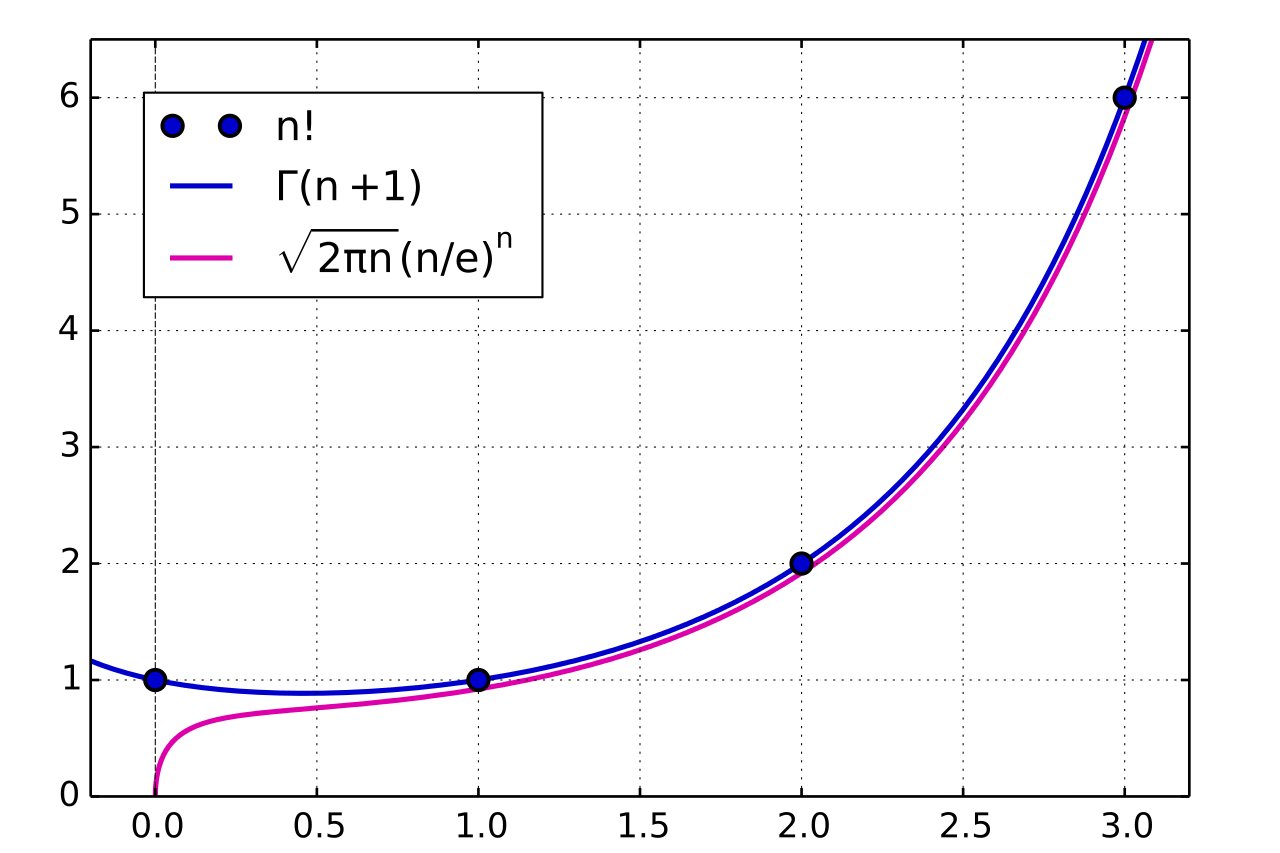
\includegraphics[scale=0.30]{figures/factorial_gamma_stirling.png}
\caption{Error de aproximaci\'on stirling respecto del factorial.}
\label{stirling_error}
\end{figure}

\pagebreak
\subsection{Código para realizar la aproximación de Stirling}
\lstinputlisting[language=Python]{../src/stirling.py}



\documentclass[12pt]{article}
\usepackage[spanish,es-tabla,es-nodecimaldot]{babel}
\usepackage{tikz}
\usepackage{amsmath, amssymb, amsbsy}    %Caracteres especiales de matematicas
\usepackage[hidelinks]{hyperref}    % Vinculos [que no estén subrayados]
\usepackage{listings}   %Introducir codigo
\usepackage{setspace}
\usepackage{color}
\usepackage{pdflscape}  %Voltear la página
\usepackage{graphicx}
\usepackage{caption}


\begin{document}
\title{Ejercicios de Técnicas de Conteo}
\author{Ana Maritza Bello Ya\~nez}
\maketitle
\setlength{\parindent}{0pt}
\setlength{\parskip}{1em}

\section*{Ejercicios de Combinatoria (Schaum)}
% Problemas 1.7, 1.8, 1.29, 1.39, 1.40, 1.77, 1.78, 1.87
% 5 ejemplos de muestras ordenadas

\subsection*{Problema 1.7}
Demostrar que un número palindrómico (decimal) de longitud par es divisible por
11.

\textbf{Solución}

La prueba inductiva explota el hecho de que cuando se quitan el primer y el
último carácter de un palíndromo, queda un palíndromo. Así, sea $N$ un número
palindrómico de longitud $2k$. Si $k = 1$, el teorema obviamente se cumple. Si
$k \geq 2$, tenemos

$ N = a_{2k-1} 10^{2k-1} + a_{2k-2} 10^{2k-2} + ... + a_{k} 10^{k} + ... +
a_{2k-2} 10^{1} + a_{2k-1} 10^{0} $

$ = a_{2k-1}(10^{2k}+10^0) + (a_{2k-2}10^{2k-2}+...+ a_{2k-2}10^{1}) $

$ \equiv a_{2k-1} P + Q$

Donde:

$P = \underbrace{100...001}_{\text{longitud } 2k} =
\underbrace{9090...9091}_{\text{longitud } 2k-2}$

y ya sea $Q=0$ (divisible por 11) o, para algún $1 \leq r \leq k-1$,

$Q = 10^r$ \{palindrome de longitud $ 2(k-r)\} = 10^r\{11R\} $

donde el último paso se sigue de la hipótesis de inducción. Por lo tanto, $N$ es
divisible por 11 y la demostración está completa.

\subsection*{Problema 1.8}

En un palíndromo binario, el primer dígito es 1 y cada dígito subsiguiente puede
ser 0 o 1. Cuente los palíndromos binarios de longitud $n$.

\textbf{Solución}

Tenemos $[(n + 1)/2] - 1 = [(n - 1)/2]$ posiciones libres, por lo tanto el número
deseado es:

$2^{[(n-1)/2]}$


\subsection*{Problema 1.29}
Encuentre la probabilidad $p_n$ de que un grupo de $n$ personas reunidas al azar
incluya al menos 2 personas con el mismo cumpleaños (día del año).

\textbf{Solución}

Aquí no tratamos con una muestra de personas, sino con una muestra de
cumpleaños, es decir, números enteros del 1 al 365 inclusivo. Nuestra noción de
probabilidad es:

$\text{Probabilidad} = \frac{\text{número de muestras favorables}}{\text{Número total de muestras}}$

En este problema es simple considerar el evento complementario: todos los $n$
cumpleaños son distintos. Este evento es realizado en $P(365,n)$ muestras; y el
total de muestras es $365^n$. Por lo tanto, $1-p_n = P(365,n)/365^n$ o:

$p_n = 1 - \frac{P(365,n)}{365^n} = 1 -
\frac{(365)(365-1)(365-2)...[365-(n-1)]}{365^n} $

$= 1-(1 - \frac{1}{365})(1 - \frac{2}{365})...(1 - \frac{n-1}{365})$

Puede verificarse que $p_n \geq 1/2 $ cuando $n>25$.

\subsection*{Ejercicio 1.39}
Pruebe que 
\begin{enumerate}
	\item 
    \begin{equation*}
		\Sigma_{r=0}^nC(n,r)=2^n
    \end{equation*}

\textbf{Solución}

\begin{eqnarray*}
	\Sigma_{r=0}^{n} \binom{n}{r}=\Sigma_{r=0}^{n} \binom{n}{r}(1^{n-r})(1^r)=(1+1)^n=2^n
\end{eqnarray*}
	
    \item 
    \begin{equation*}
		\Sigma_{r=0}^n(-1)^rC(n,r)=0
	\end{equation*}

\textbf{Solución}

\begin{eqnarray*}
	\Sigma_{r=0}^{n} (-1)^r \binom{n}{r}=\Sigma_{r=0}^{n} \binom{n}{r}(1^{n-r})(-1^r)=(1-1)^n=0
\end{eqnarray*}

\item
\begin{equation*}
	\Sigma_{r=even}^nC(n,r)=\Sigma_{r=odd}^nC(n,r)=2^{n-1}
\end{equation*}

\textbf{Solución}

\begin{eqnarray*}
	\Sigma_{r=even}^nC(n,r)=\frac{\Sigma_{r=0}^{n} \binom{n}{r}}{2}=\frac{2^n}{2}=2^{n-1}\\
	\Sigma_{r=odd}^nC(n,r)=\frac{\Sigma_{r=0}^{n} \binom{n}{r}}{2}=\frac{2^n}{2}=2^{n-1}
\end{eqnarray*}
	
\end{enumerate}

\subsection*{Ejercicio 1.39}
Obtenga nuevamente los resultados del ejercicio 1.39 con argumentos combinatorios.

\textbf{Solución}

\begin{enumerate}
	
\item Si se considera un conjunto de $n$ elementos, se pueden formar $2^n$
subconjuntos (conjunto potencia). El conjunto potencia incluye los subconjuntos
que se pueden formar con r elementos. Así:

\begin{equation*}
	|\mathcal{P}|=2^n=\binom{n}{0}+\binom{n}{1}+...+\binom{n}{n-1}+\binom{n}{n}=\Sigma_{r=0}^{n} \binom{n}{r}
\end{equation*} 

\item Se establece que X tiene tantos subconjuntos con $r$ elementos pares como
$r$ elementos impares.

Caso 1: Esto se cumple si n es impar.
	
Caso 2: Cuando $n$ es par.

Se descompone $X=X'\cup \{j\}$. Donde $j$ es un elemento de $X$\\
	
Ahora $X'$ está compuesto por un n\'umero impar de elementos, por lo que tiene
la misma cantidad de subconjuntos formados con $r$ par ($X_p$) o impar ($X_i$),
pero como se había eliminado un elemento $|X_p|=|X_i|=2^{n-1}$

\end{enumerate}

\subsection*{Ejercicio 1.77}

Muestre que en un grupo de n personas, al menos 2 personas conocen al mismo
n\'umero de personas.

\textbf{Solución}

Sea $k$ el n\'umero de personas que no conoce a nadie del grupo

\begin{itemize}
\item Caso $k>1$: Hay m\'as de una persona que no conoce a nadie y entonces se
cumple el enunciado.
	
\item Caso $k=0$: Como no hay persona que no conozca a nadie. Todas las personas
pueden conocer al menos a 1 persona o hasta $n-1$ personas. 
	
Con el principio del palomar (principio de Dirichlet), supongamos que las cajas
(pichoneras) están de acuerdo al n\'umero de personas conocidas. Es decir, que
puede haber hasta $n-1$ pichoneras y que le han preguntado a las $n-1$ personas
a cuántos de los otros conocen. En el caso extremo, uno a uno se ir\'an
colocando en las cajas correspondientes a sus n\'umeros.
	
Cuando le pregunten a la persona $n$, forsozamente tendr\'a que elegir un
n\'umero que alguien m\'as haya elegido y entonces el enunciado se cumple. 
	
\item Caso $k=1$: Se puede despreciar a esa persona que no conoce a nadie y
entonces se hace el an\'alisis para el caso k=0 con un grupo de $n-1$ personas.

\end{itemize}

\subsection*{Problema 1.78}

Considera un torneo in el cual cada uno de los $n$ jugadores juega contra cada
uno de los otros jugadores y cada jugador gana al menos 1 juego. Prueba que hay
al menos dos jugadores que tienen el mismo n\'umero de victorias.

El n\'umero de victorias de cada jugador es al menos una y por mucho $n-1$
victorias. Estos $n-1$ n\'umeros corresponde a las pichoneras para acomodar $n$
palomas.

\subsection*{Problema 1.87}
Hay 12 computadoras y 8 impresoras l\'aser en una oficina. Encuentra el n\'umero
m\'inimo de conexiones que se tienen que hacer para garantizar que si 8 o menos
computadoras quieren imprimir al mismo tiempo, cada una de ellas ser\'a capaz de
usar una impresora diferente.\\

Suponemos que las impresoras se denotan por $P_{j} (j=1,2,...,8)$ y las
computadoras por $C_{i} (i=1,2,..,12)$.\\

Conectar la primera impresora a las primeras cinco computadoras. Despu\'es
conectar la segunda impresora a las 5 impresoras consecutivas empezando por
$C_{2}$. Despu\'es conectar la tercera impresora con las 5 computadoras
consecutivas empezando por $C_{3}$ y as\'i consecutivamente para generar la
matriz de conexiones.

\begin{table}[h!]
	\begin{tabular}{l|lllllllll}
		       &$P_{1}$&$P_{2}$&$P_{3}$ &$P_{4}$&$P_{5}$&$P_{6}$&$P_{7}$&$P_{8}$&\\\hline
		$C_{1}$&  1&  0&  0&   0& 	 0&   0&   0&  0&\\ 
		$C_{2}$&  1&  1&  0&   0& 	 0&   0&   0&  0&\\
		$C_{3}$&  1&  1&  1&   0& 	 0&   0&   0&  0&\\
		$C_{4}$&  1&  1&  1&   1& 	 0&   0&   0&  0&\\
		$C_{5}$&  1&  1&  1&   1& 	 1&   0&   0&  0&\\
		$C_{6}$&  0&  1&  1&   1& 	 1&   1&   0&  0&\\
		$C_{7}$&  0&  0&  1&   1& 	 1&   1&   1&  0&\\
		$C_{8}$&  0&  0&  0&   1& 	 1&   1&   1&  1&\\
		$C_{9}$&  0&  0&  0&   0& 	 1&   1&   1&  1&\\
		$C_{10}$&  0&  0&  0&   0& 	 0&   1&   1&  1&\\
		$C_{11}$&  0&  0&  0&   0& 	 0&   0&   1&  1&\\
		$C_{12}$&  0&  0&  0&   0& 	 0&   0&   0&  1&\\
	\end{tabular}
\end{table}

Sean las 8 computadoras que requieren una impresora $C_{i_{1}}, C_{i_{2}},...,
C_{i_{8}}$ donde $i_{1} <i_{2}<...<i_{8} < $. Si 8 computadoras pueden ser
acomodadas, entonces se puede acomodar cualquier n\'umero m\'as peque\~no. La
observaci\'on crucial es:

\begin{equation}
	s \leq i_{s} \leq s+4   (s=1,2,...,8)
\end{equation}

En efecto, si $i_{s} < s$ existen $s$ enteros positivos menores que $s$ y si
$i_{s} > s+5$, al menos $12-(s+6)+1=7-s$ valores estar\'ian disponibles para los
$8-s$ indices restantes.\\


\section*{Ejercicios de Probabilidad (Schaum)}
% Problemas 2.29, 2.30, 2.68 al 2.74

\subsection*{Problema 2.29}
Construya el diagrama de árbol para las permutaciones de $\{ a,b,c \}$.

\begin{figure}[h]
	\begin{center}		
	\begin{tikzpicture}[level distance=1cm, level 1/.style={sibling distance=3cm},
		level 2/.style={sibling distance=2cm}, every node/.style={circle, draw,
		align=center} ]
				\centering
				\node[circle,draw]{$P_n$}
		child{node{a} child{node{b} child{node{c}} } child{node{c} child{node{b}}} }
		child{node{b} child{node{a} child{node{c}} } child{node{c} child{node{a}}} }
		child{node{c} child{node{a} child{node{b}} } child{node{b} child{node{a}}} };
			\end{tikzpicture}
		\end{center}
		\caption{Permutaciones para 3 elementos}
		\label{permutaciones_tree}
\end{figure}

\subsection*{Problema 2.30}

Una persona tiene tiempo para jugar a la ruleta cinco veces como máximo. En cada
jugada gana o pierde un dólar.

La persona comienza con un dólar y dejará de jugar antes de las cinco veces si
pierde todo su dinero o si gana tres dólares, es decir, si tiene cuatro dólares.
Encuentre el número de formas en que pueden ocurrir las apuestas.


El diagrama de árbol a la derecha describe la forma en que se pueden realizar
las apuestas. Cada número en el diagrama denota la cantidad de dólares que tiene
el hombre en ese momento. Observe que las apuestas pueden ocurrir de 11 maneras
diferentes. Tenga en cuenta que dejará de apostar antes de que se cumplan los
cinco tiempos en solo tres de los casos.

% Set the overall layout of the tree
\tikzstyle{level 1}=[level distance=1.5cm, sibling distance=3.5cm]
\tikzstyle{level 2}=[level distance=1.5cm, sibling distance=3.5cm]
\tikzstyle{level 3}=[level distance=1.5cm, sibling distance=3cm]
\tikzstyle{level 4}=[level distance=1.0cm, sibling distance=2.5cm]
\tikzstyle{level 5}=[level distance=1.0cm, sibling distance=0.5cm]

% Define styles for bags and leafs
\tikzstyle{bag} = [text width=1em, text centered]
\tikzstyle{end} = [circle, minimum width=0.5pt,fill, inner sep=0pt]

\begin{tikzpicture}[grow=right, sloped]
    \node[bag] {1}
    child {
        node[bag] {0}
        }
    child {
        node[bag] {2}% This is the first of three "Bag 2"
        child {
                node[bag] {3}
                child{
                        node[bag] {2}
                                                    child {
                             node[bag] {3}
                                                         child {
                             node[bag] {4}
                }
                            child {
                             node[bag] {2}
                }
                }
                            child {
                             node[bag] {1}
                                                         child {
                             node[bag] {2}
                }
                            child {
                             node[bag] {0}
                }
                }
                }
                child{
                        node[bag] {4}
                }
            }
            child {
                node[bag] {1}
                child {
        node[bag] {2}
            child {% Here are three children, hence three end branches
                node[bag] {3}
                            child {
                             node[bag] {2}
                }
                            child {
                             node[bag] {0}
                }
            }
            child {
                node[bag] {1}
                            child {
                             node[bag] {2}
                }
                            child {
                             node[bag] {0}
                }
            }
    }
            }
    }
    ;
    \end{tikzpicture}

\begin{landscape}

\subsection*{Problema 2.68}
Construye el diagrama de árbol para el número de permutaciones de $\{ a,b,c,d
\}$

\begin{tikzpicture}[
    auto,
    level 1/.style={sibling distance=58mm},
    level 2/.style={sibling distance=18mm},
    level 3/.style={sibling distance=8mm},
    ]
    \node [circle,draw] (z){}
        child {
            node[circle,draw] (b) {a}
            child { 
                node[circle,draw] (c) {b}
                child {
                    node[circle,draw] (d) {c}
                    child {
                        node[circle,draw] (e) {d}
                    }
                }
                child {
                    node[circle,draw] (d) {d}
                    child {
                        node[circle,draw] (e) {c}
                    }
                }               
            }
             child { 
                node[circle,draw] (c) {c}
                child {
                    node[circle,draw] (d) {b}
                    child {
                        node[circle,draw] (e) {d}
                    }
                }
                child {
                    node[circle,draw] (d) {d}
                    child {
                        node[circle,draw] (e) {b}
                    }
                }               
            } 
            child { 
                node[circle,draw] (c) {d}
                child {
                    node[circle,draw] (d) {b}
                    child {
                        node[circle,draw] (e) {c}
                    }
                }
                child {
                    node[circle,draw] (d) {c}
                    child {
                        node[circle,draw] (e) {b}
                    }
                }               
            }  
        }
        child {
            node[circle,draw] (b) {b}
                        child { 
                node[circle,draw] (c) {a}
                child {
                    node[circle,draw] (d) {c}
                    child {
                        node[circle,draw] (e) {d}
                    }
                }
                child {
                    node[circle,draw] (d) {d}
                    child {
                        node[circle,draw] (e) {c}
                    }
                }               
            }
                       child { 
                node[circle,draw] (c) {c}
                child {
                    node[circle,draw] (d) {a}
                    child {
                        node[circle,draw] (e) {d}
                    }
                }
                child {
                    node[circle,draw] (d) {d}
                    child {
                        node[circle,draw] (e) {a}
                    }
                }               
            }
                       child { 
                node[circle,draw] (c) {d}
                child {
                    node[circle,draw] (d) {a}
                    child {
                        node[circle,draw] (e) {c}
                    }
                }
                child {
                    node[circle,draw] (d) {c}
                    child {
                        node[circle,draw] (e) {a}
                    }
                }               
            }
        }
        child {
            node[circle,draw] (b) {c}
                        child { 
                node[circle,draw] (c) {a}
                child {
                    node[circle,draw] (d) {b}
                    child {
                        node[circle,draw] (e) {d}
                    }
                }
                child {
                    node[circle,draw] (d) {d}
                    child {
                        node[circle,draw] (e) {b}
                    }
                }               
            }
                        child { 
                node[circle,draw] (c) {b}
                child {
                    node[circle,draw] (d) {a}
                    child {
                        node[circle,draw] (e) {d}
                    }
                }
                child {
                    node[circle,draw] (d) {d}
                    child {
                        node[circle,draw] (e) {a}
                    }
                }               
            }
                        child { 
                node[circle,draw] (c) {d}
                child {
                    node[circle,draw] (d) {a}
                    child {
                        node[circle,draw] (e) {b}
                    }
                }
                child {
                    node[circle,draw] (d) {b}
                    child {
                        node[circle,draw] (e) {a}
                    }
                }               
            }
        }
        child {
            node[circle,draw] (b) {d}
                       child { 
                node[circle,draw] (c) {a}
                child {
                    node[circle,draw] (d) {b}
                    child {
                        node[circle,draw] (e) {c}
                    }
                }
                child {
                    node[circle,draw] (d) {c}
                    child {
                        node[circle,draw] (e) {b}
                    }
                }               
            }
                       child { 
                node[circle,draw] (c) {b}
                child {
                    node[circle,draw] (d) {a}
                    child {
                        node[circle,draw] (e) {c}
                    }
                }
                child {
                    node[circle,draw] (d) {c}
                    child {
                        node[circle,draw] (e) {a}
                    }
                }               
            }
                        child { 
                node[circle,draw] (c) {c}
                child {
                    node[circle,draw] (d) {a}
                    child {
                        node[circle,draw] (e) {b}
                    }
                }
                child {
                    node[circle,draw] (d) {b}
                    child {
                        node[circle,draw] (e) {a}
                    }
                }               
            }
        }
        
        ;
\end{tikzpicture}


\end{landscape}

\subsection*{Problema 2.69}


\subsection*{Problema 2.70}


\subsection*{Problema 2.71}

\subsection*{Problema 2.72}

\subsection*{Problema 2.73}

\subsection*{Problema 2.74}

\end{document}

\documentclass[12pt]{article}
\usepackage[spanish,es-tabla,es-nodecimaldot]{babel}
\usepackage{tikz}
\usepackage{amsmath, amssymb, amsbsy}    %Caracteres especiales de matematicas
\usepackage[hidelinks]{hyperref}    % Vinculos [que no estén subrayados]
\usepackage{listings}   %Introducir codigo
\usepackage{setspace}
\usepackage{color}
\usepackage{pdflscape}  %Voltear la página
\usepackage{graphicx}
\usepackage{caption}


\begin{document}
\title{Problemas de probabilidad}
\author{Ana Maritza Bello Yañez}
\maketitle
\setlength{\parindent}{0pt}
\setlength{\parskip}{1em}

\section{Problema}
Una empresa de manufactura que emplea tres planos analíticos para el diseño y
desarrollo de un productos específico. Por razones de costos los tres se
utilizan en momentos diferentes. De hecho, los planos 1, 2 y 3 se utilizan para
30\%, 20\% y 50\% de los productos respectivamente. La tasa de defectos difiere
en los 3 procedimientos de la siguiente manera,\

$P(D|P_1)=0.01 P(D|P_2)=0.03 P(D|P_3)=0.02 $ \

En donde $P(D|P_j)$ es la probabilidad de que un producto esté defectuoso, dado
el plano j.\

Si se observa un producto al azar y se descubre que está defectuoso, ¿cuál de
los planos tiene más probabilidades de haberse utilizado y, por lo tanto, de ser
el responsable?\\

\textbf{Solución} \

A partir del planteamiento del problema \

$P(P_1)=0.30, P(P_2)=0.20 y P(P_3)=0.50$ debemos calcular $P(P_j|D)$ para $j =
1, 2, 3.$

La regla de Bayes muestra que\

$P(P_1|D)=\frac{(P(P_1)P(D|P1)}{P(P_1)P(P_1|D)+P(P_2)P(D|P_2)+P(P_3)P(D|P_3)} =
\frac{(0.30)(0.01)}{(0.3)(0.01)+(0.20)(0.03)+(0.50)(0.02)}=\frac{0.003}{0.019}=0.158$\ 

De igual manera,\

$P(P_2|D) = \frac{(0.03)(0.20)}{0.019} = 0.316$ y
$P(P_3|D)=\frac{(0.02)(0.50)}{0.019}=0.526.$\

La probabilidad condicional de un defecto, dado el plano 3, es la mayor de las
tres; por consiguiente, un defecto en un producto elegido al azar tiene más
probabilidad de ser el resultado de haber usado el plano 3.

\section{Problema}
Un bit es 0 ó 1, un byte una secuencia de 8 bits. Encuentra (a) El número de
bytes (b) El número de bytes que comienzan con 11 y no terminan con 11 (c) El
número de bytes que comienzan con 11 o terminan con 11. (d) El número de bytes
que comienzan con 11 o terminan con 11

\textbf{Solución}\

(a) $2^8 = 256$.

(b) Si un byte tiene 8 bits, entonces las 4 posiciones de en medio pueden
llenarse de $2^4 = 16$ maneras. 

(c) $2^6 = 64$ bytes comienzan con 11; por lo tanto, menos los $2^4 = 16$
espacios que no terminan en 11, tenemos $64 - 16 = 48$.

(d) Si usamos (b), 64 bytes comienzan con 11; y de igual manera 64 bytes
terminan con 11. Sumándolos, tenemos 64+64 = 128, y cada byte que empieza y
termina con 11 se cuenta doble. Así, la respuesta es 128 - 16 = 112 bytes. 

\section{Problema}
Entre un grupo de programadores, 49 estudiaron Pascal. 37 estudiaron COBOL y 21
estudiaron FORTRAN. Si 9 de esos programadores estudiaron Pascal y COBOL, 5
estudiaron Pascal y FORTRAN, 4 estudiaron COBOL y FORTRAN, 3 estudiaron Pascal,
cobol y FORTRAN, ¿cuanto programadores hay en este grupo?

\textbf{Solución}

Pascal = C, Cobol = C, Fortran = F, el número de programadores en el grupo está
dado por: $|P \cup C \cup F|$.

El total de estudiantes está dado por $n_1 = |P|+|C|+|F| = 49+37+21=107$ $n_2
=|P \cap C| + |P \cap F| + |C \cap F| = 9+5+4 = 18$ $n_3 = |P \cap C \cap F| =
3$

Por lo tanto por el principio de inclusión-exclusión $|P \cup C \cup F| = n_1 - n_2 +
n_3 = 107-18+3 = 92$

\section{Problema}
¿Cuál es la probabilidad de que un número entero positivo seleccionado de un
conjunto de enteros positivos, que no excedan 100, sea divisible ya sea entre 2
o 5. 

\textbf{Solución}

Sea el $E_1$ el evento en el que el entero seleccionado es divisible entre 2, y
sea $E_2$ el evento en el que es divisible entre 5. Entonces $E_1 \cup E_2$ es
el evento en el que el número seleccionado es divisible entre 2 y entre .

Por otra parte $E_1 \cap E_2$ es el evento en el que el número seleccionado es
divisible entre 2 y entre 6, o equivalentemente, que sea divisible entre 10.

Tenemos que:
$|E_1|=50, |E_2|=20,|E_1 \cap E_2|=10,$

entonces

$p(E_1 \cup E_2)=p(E_1)+p(E_2)-p(E_1 \cap E_2) = \frac{50}{100} + \frac{20}{100} - \frac{10}{100} = \frac{3}{5}$


\section{Problema}

Los alces moran en cierto bosque. Hay $N$ alces, de los cuales se captura y
etiqueta una muestra aleatoria simple de tamaño $n$ ("muestra aleatoria simple"
significa que todos los $\binom{n}{k}$ conjuntos de $n$ alces son igualmente
probables). Los alces capturados se devuelven a la población y luego se extrae
una nueva muestra, esta vez de tamaño $m$. Este es un método importante que se
usa ampliamente en ecología, conocido como \textit{captura-recaptura}. ¿Cuál es
la probabilidad de que exactamente $k$ de los $m$ alces en la nueva muestra
hayan sido marcados previamente? (Suponga que un alce que fue capturado antes no
tiene más o menos probabilidades de ser capturado nuevamente.

\textbf{Solución}

Asumimos que todas las muestras de tamaño $m$ son igualmente probables. Para
tener exactamente k sea elk etiquetado, necesitamos elegir $k$ de los $n$ alces
etiquetados, y luego $m-k$ de los $N-n$ elk no etiquetados. Entonces la
probabilidad es

$\frac{\binom{n}{k}*\binom{N-n}{m-k}}{\binom{N}{m}}$

para $k$ tal que $0 \leq k \leq n$ y $0 \leq m-k \leq N-n$, y la probabilidad es
0 para todos los demas valores de $k$ (por ejemplo, si $k > n$ la
probabilidad es 0 ya que entonces ni siquiera hay $k$ alces etiquetados en toda
la población).

\section{Problema}

Hay 100 pasajeros en fila para abordar un avión con 100 asientos (con cada
asiento asignado a uno de los pasajeros). El primer pasajero en la fila decide
locamente sentarse en un asiento elegido al azar (con todos los asientos
igualmente probables). Cada pasajero subsiguiente toma su asiento asignado si
está disponible y, de lo contrario, se sienta en un asiento disponible al azar.

¿Cuál es la probabilidad de que el último pasajero de la fila se siente en su
asiento asignado?

\textbf{Solución}

Observemos la situación cuando entra el $k$-ésimo pasajero. Ninguno de los
pasajeros anteriores mostró preferencia por el $k$-ésimo asiento frente al
asiento del primer pasajero. Esto en particular es cierto cuando $k=n$. Pero el
$n$-ésimo pasajero solo puede ocupar su asiento o el del primer pasajero. Por lo
tanto la probabilidad es $\frac{1}{2}$.

\section{El problema de los dos mentirosos}

Los sujetos $A$ y $B$ dicen la verdad con la probabilidad de $1/3$ y mienten con
una probabilidad de $(2/3)$.

$A$ dice una declaración, y $B$ confirma que la declaración hecha por $A$ es
cierta.

¿Cuál es la probabilidad que $A$ estuviera diciendo la verdad?

\textbf{Solución}

Sea $E$ el evento en el que $A$ hace una declaración y $B$ la confirma. Esto
puede pasar de dos manetas:

\begin{itemize}
    \item $T$: $A$ y $B$, ambos dicen la verdad.
    \item $L$: $A$ y $B$, ambos están mintiendo.
\end{itemize}

$P(E)=P(T)+P(L)=\frac{1}{3}*\frac{1}{3}+\frac{2}{3}*\frac{2}{3}-\frac{5}{9}$

Dado que observamos $E$, estamos interesados en encontrar la probabilidad de que
el proceso subyacente sea, de hecho, $T$, es decir, $P(T|E)$. De la fórmula de las
probabilidades condicionales, tenemos que:

$P(T|E)=\frac{P(T \cap E)}{P(E)}$  y $P(T \cap E) = P(T)$

ya que $T \subset E$.

En conclusión:

$P(T|E) = \frac{P(T)}{P(E)} = \frac{1/9}{5/9} = \frac{1}{5}$

\section{La ameba sobreviviente}

Una población comienza con una sola ameba. Para esta y para las generaciones
posteriores, existe una probabilidad de 3/4 de que una ameba individual se
divida para crear dos amebas, y una probabilidad de 1/4 de que se extinga sin
producir descendencia. ¿Cuál es la probabilidad de que el árbol genealógico de
la ameba original continúe para siempre?

\textbf{Solución}

Esta es una caminata aleatoria sesgada disfrazada con un estado de absorción en
0 que comienza en 1. Si esta caminata aleatoria está en $N$, considerar $N$
movimientos corresponde a considerar el destino de $N$ amebas simultáneamente.
Esto produce $1-\frac{1-p}{p}=1-\frac{1/4}{3/4}=\frac{2}{3}$ por los argumentos
habituales.

\section{Duelo justo}

Pepe y Juan se han retado a un duelo. Tomarán turnos disparando uno al otro
hasta que uno sea herido. Pepe, quien puede atinarle a Juan solamente el 40\% de
las veces, es el disparador más débil, por lo que le será permitido disparar
primero. Ellos han determinado que en el duelo no se favorezca a nadie.

¿Cuál es la probabilidad de herir a Pepe?

\end{document}



\pagebreak
\section{Definiciones}

\subsection{Parámetro}

Variable y parámetro son dos términos muy utilizados en matemáticas y física.
Una variable es una entidad que cambia con respecto a otra entidad. Un parámetro
es una entidad que se utiliza para conectar variables. Los conceptos de variable
y parámetro son muy importantes en campos como las matemáticas, la física, la
estadística, el análisis y cualquier otro campo que tenga usos de las
matemáticas.

Un parámetro es una cantidad que influye en la salida o el comportamiento de un
objeto matemático, pero se considera que se mantiene constante. Los parámetros
están estrechamente relacionados con las variables y, a veces, la diferencia es
solo una cuestión de perspectiva. Se considera que las variables cambian,
mientras que los parámetros generalmente no cambian o cambian más lentamente. En
algunos contextos, uno puede imaginarse realizando múltiples experimentos, donde
las variables cambian a través de cada experimento, pero los parámetros se
mantienen fijos durante cada experimento y solo cambian entre experimentos.

Un lugar donde aparecen los parámetros es dentro de las funciones. Por ejemplo,
una función podría ser una función cuadrática genérica como $f(x)=ax2+bx+c$.
Aquí, la variable $x$ se considera como la entrada de la función. Los símbolos
$a$, $b$ y $c$ son parámetros que determinan el comportamiento de la función $f$.
Para cada valor de los parámetros, obtenemos una función diferente

\subsection{Población y muestra}

\begin{tabular}{l|p{6cm}|p{6cm}}
                & \textbf{Población}    &   \textbf{Muestra}    \\
\hline

Definición  & 	Universo de elementos que se van a estudiar.    &   Selección de
una parte de la población que se va a ser sujeto de estudio.   \\

\hline

Características &   

\begin{itemize} 
    \item Se puede clasificar según la cantidad de individuos que la conforman. 
    \item Posee variables estadísticas. 
\end{itemize}
& \begin{itemize}
    \item Forma parte de la población: debería comprender entre 5\% y 10\% para ser más
efectiva. 
    \item Los elementos deben ser aleatorios. 
    \item Debe ser representativa de la población.
\end{itemize} \\
\hline

    Objetivos & Analizar los datos recabados referentes a las características comunes que
comparten los elementos con diversos propósitos. & Estudiar el comportamiento,
características, gustos o propiedades de una parte representativa de la
población. \\

\hline

Ejemplos & \begin{itemize} \item Las personas que habitan un país.
\item La cantidad de carros en una ciudad.
\item Los estudiantes de un país.
\end{itemize} & Para el estudio del desempeño de los estudiantes de cinco
universidades de una ciudad en una materia específica, se toma como muestra a
500 estudiantes aleatoriamente (100 de cada institución) que estén cursando el
mismo nivel para que la muestra sea representativa.

\end{tabular}


\subsection{Tipos de poblaciones}

\begin{itemize} 
    \item Población finita: es aquella que se puede contar y se pueden
estudiar con mayor facilidad a sus integrantes. Por ejemplo, la cantidad de
personas inscritas en un gimnasio. 
    \item Población infinita: son inmensas poblaciones
donde se hace muy difícil contabilizar a sus integrantes, por lo que suele
tomarse en cuenta solo una porción de ella a la hora de realizar un estudio,
seleccionando así una muestra. Por ejemplo, la cantidad de granos de arena en
una playa. 
    \item Población real: son grupos de integrantes tangibles. Por ejemplo, la
cantidad de animales en un zoológico.
\end{itemize}

\subsection{Tipos de muestras}

\textbf{Muestreo aleatorio}. Es una técnica que ofrece la misma posibilidad a los
elementos de ser seleccionados, por ser tomados al azar. Los tipos de muestreo
aleatorio son:

\begin{itemize}

    \item Muestreo aleatorio simple: los elementos se eligen de una lista al azar.
Funciona más eficazmente cuando el universo es reducido y homogéneo. 

\item Muestreo sistemático: el primer elemento se elige al azar y luego se
escogen a intervalos constantes los elementos restantes. 

\item Muestreo estratificado: se realiza dividiendo a la población en partes o
estratos que respondan a características establecidas y luego se eligen
aleatoriamente los individuos que se van a estudiar. 

\item Muestreo por conglomerado: la población se divide en grupos heterogéneos y
éstos a su vez se subdividen en grupos homogéneos con características comunes
para ser estudiados de acuerdo a lo requerido por el investigador.
\end{itemize}

\textbf{Muestreo no aleatorio o por selección intencionada} Se elige con
base en el manejo de información de los elementos a estudiar, por lo que la
representatividad de la muestra puede ser subjetiva. En este caso, se corre el
riesgo de que los resultados sean sesgados.

\section{Variable aleatoria}

Una variable es una entidad que cambia en un sistema dado. Considere un ejemplo
simple de una partícula en movimiento a través del espacio. En tal caso,
entidades como el tiempo, la distancia recorrida por la partícula, la dirección
de viaje se denominan variables.

Hay dos tipos principales de variables en un experimento dado. Estas se conocen
como variables independientes y variables dependientes. Las variables
independientes son las variables que se cambian o que son naturalmente
inmutables. En un ejemplo simple, si se mide la tensión de una banda elástica
mientras se cambia la tensión de la banda, la tensión es la variable dependiente
y la tensión es la variable independiente. La dependencia se aplica cuando la
variable dependiente es dependiente de la variable independiente.

Las variables también se pueden categorizar como variables discretas y variables
continuas. Esta clasificación se utiliza principalmente en matemáticas y
estadística. Los problemas se pueden categorizar dependiendo del número de
variables. El número de variables es muy importante en campos como las
ecuaciones diferenciales y la optimización.

Una variable aleatoria $X$ es una función definida sobre el espacio muestral
$\omega$ (conjunto de los resultados de un experimento aleatorio) que toma
valores en el cuerpo de los números reales $mathbb{R}$, es decir:


$ X : \omega \rightarrow \mathbb{R} $


Una variable aleatoria puede ser discreta o continua según sea el rango de esta
aplicación.

%\subsection{Variable aleatoria discreta}

Una \textbf{variable aleatoria es discreta} si toma un número de valores finito
o infinito numerable. Estas variables corresponden a experimentos en los que se
cuenta el número de veces que ha ocurrido un suceso.

%\subsection{Variable aleatoria continua}

Una \textbf{variable aleatoria es continua} cuando puede tomar cualquier valor
de un intervalo real de la forma $(a, b)$,$(a,\infty)$,$(-\infty, b)$,$(-\infty,
+\infty)$ o uniones de ellos. Por ejemplo, el peso de una persona, el tiempo de
duración de un suceso, etc.



\section{Probabilidad y conteo}

\subsection{Definici\'on cl\'asica}

La definici\'on cl\'asica de la probabilidad \cite{faber2012statistics} de un
evento $A$, puede ser formulada de la siguiente manera:

\begin{equation}
    P(A)= \frac{n_A}{n_(total)}
\end{equation}

Donde $n_A$ es el n\'umero de formas igualmente probables por las cuales un
experimento puede conducir a A; $n_(total)$ n\'umero total de formas igualmente
probables en el experimento.

- En la definici\'on cl\'asica el experimento no necesariamente se lleva a cabo
ya que la respuesta es conocida de antemano.

- La teor\'ia cl\'asica no da soluci\'on a menos de que todas las formas
igualmente posibles puedan ser derivadas anal\'iticamente.



\section{Probabilidad Condicional}

La probabilidad condicional nos provee una forma de razonar acerca de la salida
o resultado de un experimento, basado en información parcial. Algunos ejemplos
de estos experimentos podrían ser los siguientes:

\begin{itemize}
\item En un experimento en el cual tiramos dos dados sucesivamente, te dicen que
la suma de los dados es 9. ¿Qué tan probable es que el primer dado haya caído 6?

\item En un juego de adivinanzas de palabras, la primera letra de la palabra es
\textit{t}. ¿Cuál es la probabilidad de que la siguiente palabra sea \textit{h}?

\item ¿Qué  tan probable es que una persona tenga cierta enfermedad dado que su
examen médico dió negativo?
\end{itemize}

En términos más precisos, dado un experimento, un espacio de muestreo y una ley
de probabilidad, suponiendo que sabemos que la salida está dentro de un evento
dado $B$. Deseamos cuantificar la probabilidad de que la salida pertenece a
algún otro evento $A$. Así, podemos construir una nueva probabilidad que tome en
cuenta el conocimiento disponible: una ley de probabilidad para cuaquier evento
$A$. Especificamente, la probabilidad condicional de $A$ dado $B$, denotado por
$P(A|B)$.

Para calcular $P(A|B)$ consideramos aquellos resultados del evento $A$ que están en
el evento $B$. Esto nos da los resultados en el evento $A \cap B$ y nos lleva al
teorema de la probabilidad condicional.

\begin{theorem}{Probabilidad Condicional}{conditional_probability}
Sea $S$ el espacio de muestro para un experimento $E$ y $A$, $B \subseteq S$,
entonces la probabilidad condicional de $A$ dado $B$ está dada por:
    \begin{equation}
        P(A|B) = \frac{P(A \cap B)}{P(B)}
        \label{eq:conditionalProbability}
    \end{equation}

Siempre que $P(B)>0$.

Particularmente, todas las propiedades de las leyes de la probabilidad
permanecen válidas para las leyes de la probabilidad condicional.

\begin{itemize}
    \item La probabilidad condicional puede verse también como una ley de
    probabilidad en un nuevo universo $B$, ya que toda la probabilidad condicional
    está concentrada en $B$.

    \item Si todos los resultados son finitos e igualmente probables, entonces:
        \begin{equation}
            P(A|B)=\frac{\text{número de elementos de }A \cap B}{\text{número de elementos de }B}
        \end{equation}
\end{itemize}
\end{theorem}


\def\firstcircle{(0,0) circle (1.5cm)}
\def\secondcircle{(0:2cm) circle (1.5cm)}
\def\rectangle{(-2,-2) rectangle (4,2)}

\colorlet{circle edge}{black!50}
\colorlet{circle area}{gray!20}

\tikzset{filled/.style={fill=circle area, draw=circle edge, thick},
    outline/.style={draw=circle edge, thick}}

\setlength{\parskip}{5mm}

\begin{figure}[h]
    \centering
    \begin{tikzpicture}
        \draw \rectangle;
        \begin{scope}
            \clip \firstcircle;
            \fill[filled] \secondcircle;
        \end{scope}
        \draw[outline] \firstcircle node {$A$};
        \draw[outline] \secondcircle node {$B$};
        \node[anchor=south] at (current bounding box.south) {$A \cap B$};
        \node at (3.5,1.5){$\mathbb S$};
    \end{tikzpicture}
    \caption{Representación del concepto intuitivo de la probabilidad condicional.}
    \label{fig:coditionalProbability}
\end{figure}

\def\firsttcircle{(90:1.75cm) circle (1.5cm)}
\def\seconddcircle{(170:1.75cm) circle (1.5cm)}
\def\thirddcircle{(-25:2cm) circle (1.5cm)}
\begin{figure}
    \centering
\begin{tikzpicture}
      \begin{scope}
    \clip \seconddcircle;
    \fill[cyan] \thirddcircle;
      \end{scope}
      \begin{scope}
    \clip \firsttcircle;
    \fill[cyan] \thirddcircle;
      \end{scope}
      \draw \firsttcircle node[text=black,above] {$A$};
      \draw \seconddcircle node [text=black,below left] {$B$};
      \draw \thirddcircle node [text=black,below right] {$C$};
\end{tikzpicture}
\end{figure}

\textbf{Observaciones y consideraciones de la probabilidad condicional:}

\begin{itemize}
\item La probabilidad $P(A|B)$ es una actualización de $P(A)$, basada en el
conocimiento de que ocurrió el evento $B$.

\item De la Ec.(\ref{eq:conditionalProbability}), tanto $P(A \cap B)$ como
$P(A)$ se calculan a partir del espacio muestral original.

\item Las probabilidades tienen sutiles cambios dependiendo de la información
exacta de la condición implicada en el evento A.
\end{itemize}

\subsection{Propiedades de las leyes de la probabilidad}

Las leyes de la probabilidad tienen propiedades que pueden deducirse de los
axiomas. Algunas de ellas, son las que se muestran a continuación.

\begin{tcolorbox}[colback=blue!5!white,colframe=blue!60!black,title=Resumen: Propiedades de las leyes de la probabilidad]
    Sean $A$, $B$ y $C$ eventos:

    \begin{itemize}
        \item Si $A \subset B$, entonces $P(A) \leq P(B)$.
        
        \item $P(A \cup B) = P(A) + P(B) - P(A \cap B)$.

        \item $P(A \cup B) \leq P(A) + P(B)$.

    \item $P(A \cup B \cup C) = P(A) + P(B) + P(C) - P(A \cap B) - P(A \cap C) - P(B
        \cap C) + P(A \cap B \cap C)$
    \end{itemize}
\end{tcolorbox}

De la Ec.(\ref{eq:conditionalProbability}) podemos hacer que:

\begin{center}
$P(B \cap A) = P(A \cap B) = P(A)P(B|A)$, 
\end{center}

y cambiando los roles de $A$ y de $B$, tenemos que:

\begin{center}
    $P(A \cap B) = P(B \cap A) = P(B)P(A|B)$, 
\end{center}

esto resulta en:

\begin{center}
    $P(A)P(B|A) = P(A \cap B) = P(B)P(A|B)$,
\end{center}

Que comunmente llamamos \textit{regla de la multiplicación}.

\begin{figure}
% Set B but not A
\centering
\begin{tikzpicture}
    \draw \rectangle;
    \begin{scope}
        \clip \secondcircle;
        \draw[filled, even odd rule] \firstcircle
                                     \secondcircle node {$B$};
    \end{scope}
    \draw[outline] \firstcircle node {$A$}
                   \secondcircle;
    \node[anchor=south] at (current bounding box.north) {$A^c \cap B$};
    \node at (1,0){$A \cap B$};
\end{tikzpicture}
\caption{Representación gráfica de la diferencia de los conjuntos de $A-B$ y de $B-A$.}
\label{fig:difer}
\end{figure}

\subsection{Teorema de Bayes}

\begin{theorem}{Teorema de Bayes}{BayesTheorem}
Sean $A$ y $B$ dos eventos cuyas probabilidades son diferentes de cero,
entonces:
    \begin{equation}
        P(B|A) = \frac{P(A|B) P(B)}{P(A)}
        \label{eq:BayesTheorem}
    \end{equation}

La implicación más importante de la Ec. (\ref{eq:BayesTheorem}) es que permite
encontrar probabilidades condicionadas $P(B|A)$ en términos de $P(A|B)$, cuando
esta última resulta más fácil de calcular directamente.
\end{theorem}



\section*{Convenio de suma de Einstein}

Se denomina notación de Einstein o notación indexada a la convención utilizada
para abreviar la escritura de las sumatorias, donde se suprime el término de la
sumatoria $(\sum)$. Este convenio fue introducido por Albert Einstein en 1916.

Dada una expresión lineal en $\mathbb{R^{n}}$ en la que se escriban todos sus
términos en forma explícita:

\begin{equation}
    u = u_1 x_1 + u_2 x_2 + ...u_n x_n
\end{equation}

Se puede escribir de la forma:

\begin{equation}
    u = \sum_{i=1}^{n} u_ix_i
\end{equation}

La notación de Einstein obtiene una expresión aún más condensada eliminando el
signo de la sumatoria y entendiendo que la expresión resultante en un índice
indica la suma sobre todos los posibles valores del mismo.

\begin{theorem}{Convenio de la suma de Einstein}{convenioSuma}
    \begin{equation}
        u = u_ix_i
    \end{equation}
\end{theorem}

\subsection*{Tensor Levi-Civita}

Está definido por:

\begin{theorem}{Tensor de Levi-Civita}{leviCivita}
\begin{equation}
    \epsilon_{ijk}=
    \left\lbrace\begin{array}{ccccl} 
        +1 & ijk, & kji, & jki & \text{Permutación cíclica o par}\\ 
        -1 & ikj, & kji, & jik & \text{Permutación anticíclica o impar}\\
        0  & iii, & jjj, & kkk & \text{Si se repiten}
    \end{array}\right.
\end{equation}
\end{theorem}

\subsection*{Producto escalar de dos vectores}

También conocido como producto punto, es una operación algebraíca que toma dos
vectores y retorna un escalar. esta definido de la siguiente manera:

\begin{theorem}{Producto escalar de dos vectores}{productoEscalar}
    \begin{equation}
        \bar{A} \cdot \bar{B}= \bar{\abs{A}} \bar{\abs{B}} \cos \theta
        = \sum_{i=1}^{n} a_i b_i
    \end{equation}
\end{theorem}

Que de acuerdo al convenio de suma de Einstein podemos escribir como:

\begin{equation}
    \bar{A} \cdot \bar{B} = a_i b_i
\end{equation}

\subsection*{Producto vectorial de dos vectores}

EL producto vectorial o producto cruz de dos vectores es una operación binaria
entre dos vectores en un espacio tridimensional. El resultado es un vector
perpendicular a los vectores que se multiplican, y por lo tanto normal al plano
que los contiene.

Está definido de la siguiente manera:

\begin{theorem}{Producto Vectorial de dos vectores}{productoVectorial}
\begin{equation}
    \bar{A} \times \bar{B}= \bar{\abs{A}} \bar{\abs{B}} \sin \theta \  \hat{r}
\end{equation}
\end{theorem}

Donde $\hat{r}$ es el vector unitario y ortogonal a los vectores $\bar{A}$ y
$\bar{B}$, y $\theta$ el ángulo entre $\bar{A}$ y $\bar{B}$.

Que mediante determinantes tenemos:

\begin{equation}
    \bar{A} \times \bar{B}=
    \begin{bmatrix}
        \hat{i} & \hat{j} & \hat{k}\\ 
         a_1 & a_1 & a_1\\ 
         b_1 & b_1 & b_1
    \end{bmatrix}
\end{equation}

Desarrollamos:

\begin{equation}
    \bar{A} \times \bar{B}= \hat{i}(a_2 b_3 - a_3 b_2) - \hat{j}(a_1 b_3 - a_3 b_1) + \hat{k}(a_1 b_2 - a_2 b_1)
\end{equation}

Desde un punto de vista tensorial el producto generalizado de $n$ vectores vendrá
dado por:

\begin{theorem}{Generalización del producto vectorial desde el punto de vista tensorial}{productoTensorial}
    \begin{equation}
        (\bar{A} \times \bar{B})_{i} = \epsilon_{ijk} a_{j} b_{k}
    \end{equation}
\end{theorem}

Desarrollando:

\begin{equation}
    \epsilon_{ijk} a_{jbk} =
    \begin{array}{ccccc}
        \cancel{\epsilon_{111} a_1 b_1} & + & \cancel{\epsilon_{112} a_1 b_2}   & + & \cancel{\epsilon_{112} a_1 b_3}   \\
        \cancel{\epsilon_{121} a_2 b_1} & + & \cancel{\epsilon_{122} a_2 b_2}   & + & \epsilon_{123} a_2 b_3            \\
        \cancel{\epsilon_{131} a_3 b_1} & + & \epsilon_{132} a_3 b_2            & + & \cancel{\epsilon_{133} a_3 b_3}
    \end{array}
    = a_2 b_3 - a_3 b_2
\end{equation}



\subsection{Congruencia de Zeller}

\lstinputlisting[language=Python]{../src/zeller_congruency.py}



\section{Matriz de rotaci\'on}
La matriz de rotación es la siguiente:
%CORREGIR


	\begin{eqnarray*}
		x^{'m} = a^{m}\hfill_{\nu} x^{\nu}\\
		m = 0,1,2,3\\
		\nu = 0,1,2,3
	\end{eqnarray*}		
	\begin{eqnarray*}
		x^{'(0)} =
		\left( {\begin{array}{cc}
				a^{0} _0 x^{_0} + a^{0} _1 x^{_1} + a^{0} _2 x^{_2} + a^{0} _3 x^{_3}\\
		\end{array} } \right)\\
	x^{'(1)} =
	\left( {\begin{array}{cc}
			a^{1} _0 x^{_0} + a^{1} _1 x^{_1} + a^{1} _2 x^{_2} + a^{1} _3 x^{_3}\\
	\end{array} } \right)\\
	x^{'(2)} =
	\left( {\begin{array}{cc}
			a^{2} _0 x^{_0} + a^{2} _1 x^{_1} + a^{2} _2 x^{_2} + a^{2} _3 x^{_3}\\
	\end{array} } \right)\\
	x^{'(3)} =
	\left( {\begin{array}{cc}
			a^{3} _0 x^{_0} + a^{3} _1 x^{_1} + a^{3} _2 x^{_2} + a^{3} _3 x^{_3}\\
	\end{array} } \right)
	\end{eqnarray*}
\begin{equation*}
	\left(
	\begin{array}{ccc}
		x^{'0}\\
		x^{'1}\\
		x^{'2}\\
		x^{'3}\\ 
	\end{array}
	\right)
	=
	\left(
	\begin{array}{c}
		a^{m}\nu
	\end{array}
	\right)
	{}
	\left(
	\begin{array}{ccc}
		x^{0}\\
		x^{1}\\
		x^{2}\\
		x^{3}\\ 
	\end{array}
	\right)
\end{equation*}		
%\caption{Matriz de rotaci\'on}
%\label{permutaciones_tree}

\chapter{Matrices de rotaci\'on}
	Una matriz de rotaci\'on es una matriz que representa una rotaci\'on en el espacio euclidiano.
	Las matrices de rotaci\'on pueden ser en dos o tres dimensiones.
	
	Por ejemplo, si la matriz de rotaci\'on es de dos dimensiones y se busca rotar en sentido horario, la matriz tendrá la siguiente forma:
	\begin{equation}
		R(\theta)=
		\begin{bmatrix}
			\cos \theta & -\sin \theta\\
			\sin \theta & \cos \theta
		\end{bmatrix}
	\end{equation}
	De esta manera, las nuevas coordenadas, una vez aplicando la rotación son de la siguiente manera:
	\begin{eqnarray}
		\left(
		\begin{matrix}
			x'\\
			y'
		\end{matrix}
		\right)
		=
		\begin{bmatrix}
			\cos \theta & -\sin \theta\\
			\sin \theta & \cos \theta
		\end{bmatrix}
		\left(
		\begin{matrix}
			x\\
			y
		\end{matrix}
		\right)\\
		x'=x\cos \theta -y\sin \theta\\
		y'=x\sin \theta + y \cos \theta
	\end{eqnarray}

En caso de querer que la rotación sea antihoraria, se utiliza la siguiente matriz:
\begin{equation}
	R(-\theta)=
	\begin{bmatrix}
		\cos \theta & \sin \theta\\
		-\sin \theta & \cos \theta
	\end{bmatrix}
\end{equation}

Si lo que se busca es realizar rotaciones en el espacio tridimensional, se deben modificar las matrices de la siguiente manera:
\begin{equation}
	R_x(\theta)=
	\begin{bmatrix}
		1 & 0 & 0\\
		0 & \cos \theta & \sin \theta\\
		0 & -\sin \theta & \cos \theta
	\end{bmatrix}
\end{equation}

\begin{equation}
	R_y(\theta)=
	\begin{bmatrix}
		\cos \theta & 0 & \sin \theta\\
		0 & 1 & 0\\
		-\sin \theta & 0 & \cos \theta
	\end{bmatrix}
\end{equation}

\begin{equation}
	R_z(\theta)=
	\begin{bmatrix}
		\cos \theta & -\sin \theta & 0\\
		\sin \theta & \cos \theta & 0\\
		0 & 0 & 1
	\end{bmatrix}
\end{equation}
\subsection{Ángulos de Euler}


Los ángulos de Euler constituyen un conjunto de tres coordenadas angulares que
sirven para especificar la orientación de un sistema de referencia de ejes
ortogonales, normalmente móvil, respecto a otro sistema de referencia de ejes
ortogonales normalmente fijos.

Dados dos sistemas de coordenadas $xyz$ y $XYZ$ con origen común, es posible
especificar la posición de un sistema en términos del otro usando tres ángulos
$\alpha$, $\beta$, $\gamma$.

La definición matemática es estática y se basa en escoger dos planos, uno en el
sistema de referencia y otro en el triedro rotado. En el esquema adjunto serían
los planos $xy$ y $XY$. Escogiendo otros planos se obtendrían distintas convenciones
alternativas, las cuales se llaman de Tait-Bryan cuando los planos de referencia
son no-homogéneos (por ejemplo $xy$ y $XY$ son homogéneos, mientras $xy$ y $XZ$ no lo
son).

La intersección de los planos coordenados $xy$ y $XY$ escogidos se llama línea de
nodos, y se usa para definir los tres ángulos, Fig. (\ref{fig:euler_angles}) :

\begin{itemize}
    \item $\alpha$ es el ángulo entre el eje $x$ y la línea de nodos.
    \item $\beta$  es el ángulo entre el eje $z$ y el eje $Z$.
    \item $\gamma$  es el ángulo entre la línea de nodos y el eje X.
\end{itemize}

Más adelante se establecerá que los tres ángulos de Euler descritos son los
valores de las tres rotaciones intrínsecas que describen el sistema.

Notar que también se considera la notación: $\alpha =\phi$, $\gamma =\psi$,
$\beta =\theta$

Las rotaciones de Euler son los movimientos resultantes de variar uno de los
ángulos de Euler dejando fijo los otros dos. Son los siguientes:

\begin{itemize}
    \item Preseción
    \item Nutación
    \item Rotación intrínseca
\end{itemize}

Si escribimos la rotación de ángulos $\phi$
,$\theta$ ,$\psi$ como una composición de estas tres rotaciones:

\begin{equation}
    A(\phi ,\theta ,\psi )=R(\phi ,\theta ,\psi )N(\phi ,\theta )P(\phi)\
\end{equation}

entonces se cumple:

\begin{equation}
    \begin{array}{ll}
    A(\delta \phi +\phi ,\theta ,\psi ) & = P(\delta \phi )A(\phi ,\theta ,\psi) \\
    A(\phi ,\delta \theta +\theta ,\psi ) & = N(\phi ,\delta \theta )A(\phi ,\theta ,\psi ) \\
    A(\phi,\theta ,\delta \psi +\psi ) &=R(\phi ,\theta ,\delta \psi )A(\phi ,\theta ,\psi) \\
    \end{array}
\end{equation}

Como consecuencia de estas propiedades, estas rotaciones son conmutativas
entre ellas:

\begin{equation}
    P(\delta \phi )N(\delta \theta )A(\phi ,\theta ,\psi)=A(\delta \phi +\phi ,\delta \theta +\theta ,\psi )=N(\delta \theta )P(\delta \phi )A(\phi ,\theta ,\psi )
\end{equation}

lo que también podría verse intuitivamente usando la analogía entre los ángulos
de Euler y los de un soporte Cardán.

\begin{figure}[h!]
	\begin{center}
		\threedalphabetagamma
	\end{center}
	\caption{Posicionamiento del marco de coordenadas girado $(x', y', z')$ 
	usando ángulos de Euler $(\alpha, \beta, \gamma)$.}
	\label{fig:euler_angles}
\end{figure}




\pagebreak
\section{Teorema de la incompletitud matemática de Gödel}

\begin{wrapfigure}{l}{0.4\textwidth}
    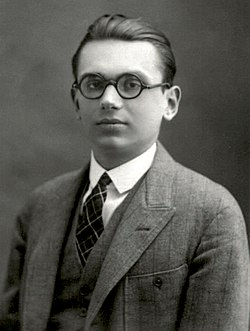
\includegraphics[width=5cm]{figures/Kurt_Godel.jpg}
    \caption{Gödel como estudiante a los 19 años de edad, 5 años antes de la 
    demostración de los teoremas.}
\end{wrapfigure}

Gödel, nacido el 28 de abril de 1906 en Brno (hoy parte de la República Checa),
demostró como parte de su tesis doctoral, en 1929, el primer teorema de
incompletitud, que afirma que todo sistema axiomático coherente que englobe las
propiedades aritméticas básicas de los números naturales padece una dicotomía
\footnote{División de un concepto o una materia teórica en dos aspectos,
especialmente cuando son opuestos o están muy diferenciados entre sí.}
fundamental: o bien no se puede implementar en un algoritmo, o bien los axiomas
no son capaces de determinar la veracidad de todos los enunciados posibles.
Gödel demostró que en todo “universo matemático” imaginable habrá propiedades
que no podemos demostrar.

Los enunciados matemáticos indecidibles son imposibles de evitar. Un ejemplo es
la hipótesis del continuo, que afirma que todo subconjunto infinito de los
números reales se puede identificar con los números naturales o con los reales.
Otro ejemplo es el axioma de elección, que afirma que dada una colección de
cajas (o conjuntos) no vacías, es posible escoger un elemento de cada caja.
Puede resultar sorprendente que este axioma sea problemático, sobre todo si sólo
pensamos en un número finito de cajas. Sin embargo, en un contexto infinito,
tiene consecuencias inesperadas: Stefan Banach y Alfred Tarski demostraron
partiendo de dicho axioma que se puede descomponer una bola de madera maciza en
un número finito de piezas, las cuales, recolocadas de cierta manera, dan como
resultado dos bolas del mismo volumen.

El teorema de Gödel o teorema de incompletitud limita las posibilidades de las
matemáticas de demostrar fórmulas a través de la deducción. Dibuja el límite a
lo que es posible conocer a través de la lógica formal tal y como se plantea en
física y otras disciplinas.  Muy resumidamente hablando, el teorema de Gödel
viene a decir que «no se puede demostrar cualquier fórmula matemática, aunque
sea verdadera».

La demostración del teorema de incompletitud se apoya en dos ideas claves: por
un lado, Gödel tuvo la destreza de codificar frases y enunciados a través de
números. Al hablar de números, ahora hablamos también de enunciados. Por otro
lado, utilizó un argumento diagonal semejante al que usó Georg Cantor para
demostrar que, pese a que hay tantos números racionales como naturales, hay
muchos más números reales que naturales.

A raíz de los trabajos de Gödel se consolidaron diversas disciplinas dentro de
la lógica matemática: por un lado, la teoría de conjuntos como paradigma de un
formalismo autosuficiente, la teoría de la recursión y de la demostración, con
un enfoque sintáctico y algorítmico, así como la teoría de modelos, en la que
trabajamos los autores de este artículo, que se concentra en las propiedades
semánticas de los objetos matemáticos.

David Hilbert (1862-1943) se preguntaba si las matemáticas eran completas,
consitentes y decidibles.

El teorema de la incompletitud de Gödel significa que la verdad y la
demostrabilidad no son lo mismo en absoluto. Hilbert estaba equivocado. Siempre
habrá afirmaciones verdaderas sobre la matemática que no podamos demostrar.

También demostro que la matemática no es consistente (libre de contradicciones),
ya que cualquier sistema formal consistente de la matemática es incapaz de
probar su propia consistencia (paradojas de autoreferencia). Así que tomando
ambos teoremas de la incompletitud de Gödel, estos dicen que lo mejor a lo que
podemos aspirar es a un sistema consistente pero incompleto de la matemática.
Pero un sistema coo ese no puede probar su propia consistencia, por lo que
algunas contradicciones podrían surgir en el futuro revelando que el sistema en
el que se trabaja ha sido inconsistente todo el tiempo.

% Eso nos deja la tercera y última pregunta de Hilbert; ¿es la matemática
% decidible?, ¿Hay algún algoritmo que pueda siempre determinar si una afirmación
% surge de los axiomas?.


% doxygen



\section{Axiomas de Peano}\label{sect: Axiomas de Peano}
Los axiomas de Peano son un sistema de postulados para la aritmética ideados por el matem\'atico Giuseppe Peano en el siglo XIX para definir los n\'umeros naturales.

Estos axiomas fueron publicados en 1889 en un art\'iculo denominado \textit{Aritmetices principia, nova methodo exposita}.

Los cinco axiomas son los siguientes:
\begin{enumerate}
	\item $N(1)$: El \textbf{1} es un n\'umero natural.
	\item $\forall x(N(x)\to N(x'))$:Todo n\'umero natural, tiene un sucesor \textbf{$n^*$}
	\item $\neg \exists x(N(x)\land 1=x')$: El \textbf{1} no es el sucesor de ning\'un n\'umero natural.
	\item $\forall x \forall y ((N(x)\land N(y)\land x'=y')\to x=y)$: Si hay dos n\'umeros naturales n y m con el mismo sucesor, entonces n y m son el mismo n\'umero natural.
	\item $\left(\phi(1)\land \forall x(\phi(x)\to \phi(x'))\right) \to \forall x \phi(x)$: Si el 1 pertenece a un conjunto de n\'umeros naturales, y dado un elemento cualquiera, el sucesor tambi\'en pertenece al conjunto. Entonces, todos los n\'umeros naturales pertencen a ese conjunto.
\end{enumerate}

Cabe mencionar que el axioma 5 es el principio de la inducci\'on matem\'atica.

Existe un debate para determinar si el $0$ pertenece o no al conjunto de los n\'umeros naturales. Sin embargo, se tomar\'a en cuenta dependiendo de la aplicaci\'on. Es por esa raz\'on que los 5 axiomas existen en la versi\'on donde el $0$ es el n\'umero natural. As\'i, los axiomas 1 al 5, donde se indique el n\'umero 1, se cambia por el 0.

Adem\'as de sus 5 axiomas, Peano define la suma y la multiplicaci\'on:
\begin{itemize}
	\item suma
	\begin{eqnarray*}
		\forall n(n+1=n')\\
		\forall n\forall m(n+m'=(n+m)')
	\end{eqnarray*}
	\item Multiplicaci\'on
	\begin{eqnarray*}
		\forall n(nx1=n)\\
		\forall n \forall m(nxm'=(nxm)+n)
	\end{eqnarray*}
\end{itemize}
De igual manera, cuando interviene el 0, \'este se colocar\'a en lugar del 1.

\newpage
\section{Ley de Benford}
\subsection*{Introducción}
En 1981, Simon Newcomb publicó un art\'iculo que comienza diciendo que la
frecuencia de aparición de los 10 dígitos en algún número no era equitativa y
que esto debía ser evidente al observar las tablas de logaritmos y notar que las
primeras p\'aginas estaban m\'as que las del final. Esto result\'o para Newcomb
en el siguiente enunciado:

\textit{La ley de probabilidad de ocurrencia de los n\'umeros es tal que la mantisa 
de su logaritmo es equiprobable.}

Despu\'es de estos resultados, en 1937, Frank Benford retoma los resultados de
Newcomb y publica su \textit{Ley de los n\'umeros an\'omalos}.

El m\'etodo de estudio consiste en seleccionar cualquier tabla de datos que no
esté restringida en rango numérico o condicionada de alguna manera y hacer el
conteo del n\'umero de veces que los n\'umeros naturales del 1 al 9 curren como
primer dígito. Si aparece un punto decimal o un cero antes del primer n\'umero
natural, estos deben ser ignorados.
\subsection*{Ley para n\'umeros grandes}
Para comrpobar su hip\'otesis, Benford recolectó informaci\'on de distintas
fuentes. Estos datos se encuentran naturalmente de forma aleatoria. Una vez que
realizó el conteo de aproximadamente 20,229 observaciones, obtuvo el promedio de
apariciones de cada dígito en la primera posici\'on de los n\'umeros
Fig. (\ref{T1Benford}). 

\begin{figure}[h]
	\centering
	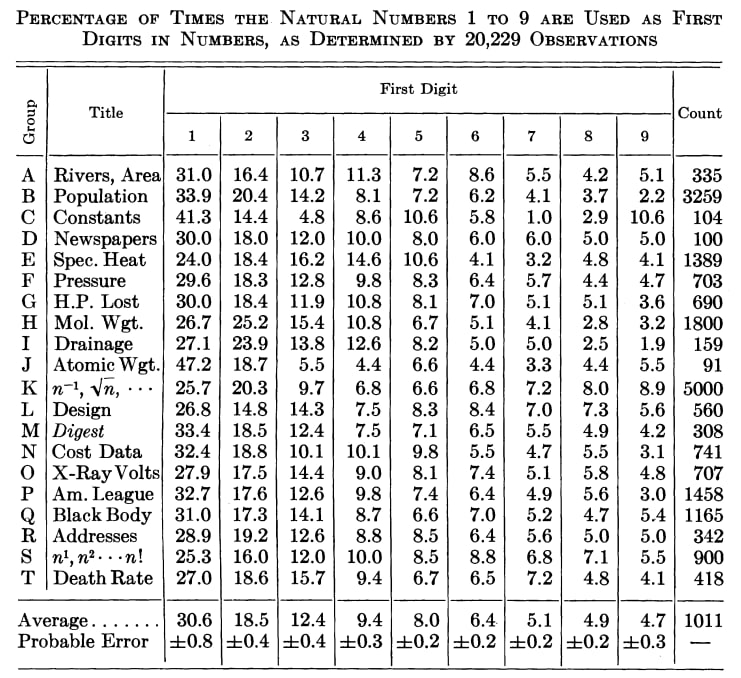
\includegraphics[scale=0.4]{figures/benford_table.jpg}
	\caption{Tabla de porcentajes de aparici\'on de los n\'umeros naturales para diferentes experimentos.}
	\label{T1Benford}
\end{figure}

\begin{figure}[h]
	\centering
	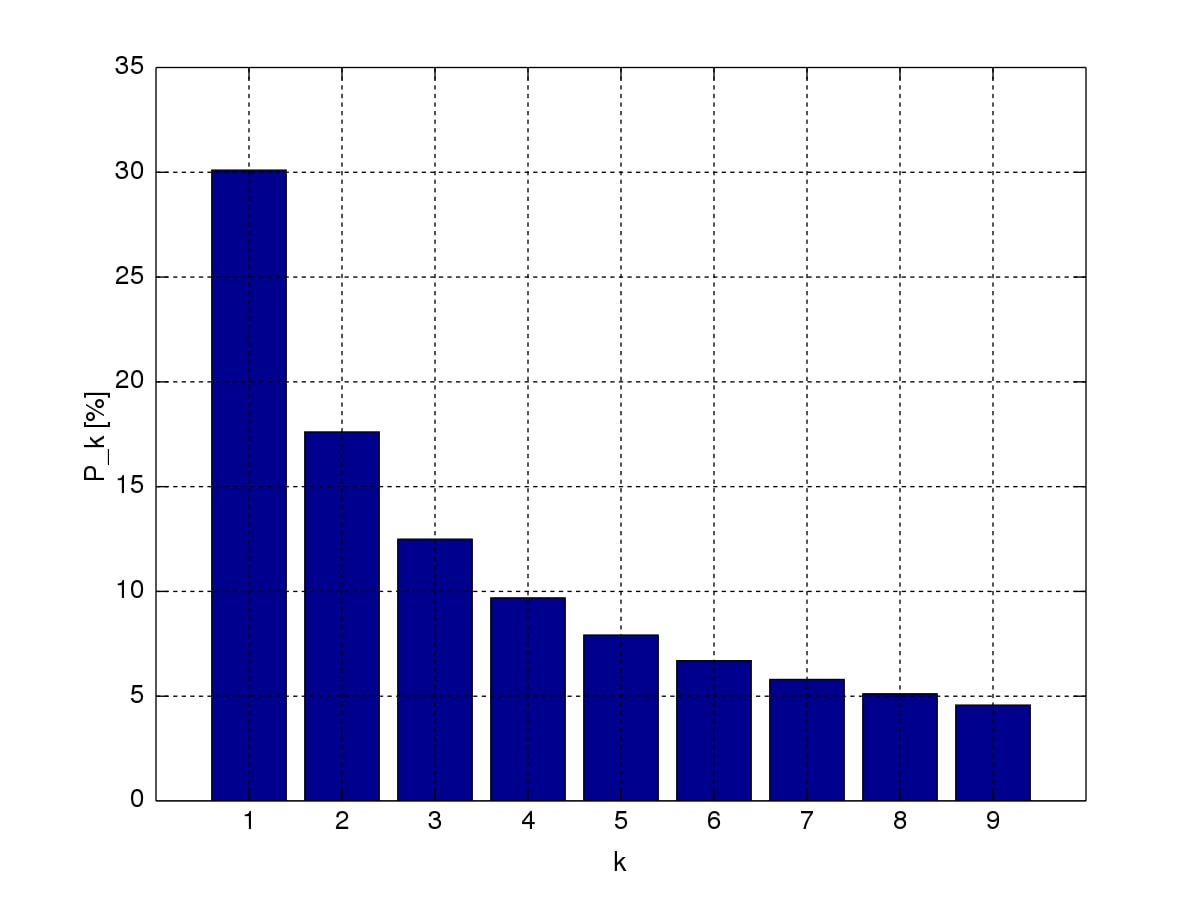
\includegraphics[scale=0.4]{figures/benford_frequency.jpg}
\caption{Gr\'afica de comportamiento para la Ec\eqref{BenfordFrecuency}.}
	\label{G1Benford}
\end{figure}
De la Fig. (\ref{T1Benford}), si se toma el promedio final de cada columna y se
estudia, por ejemplo, el 0.306, en lugar de 30.6. Se debe notar que la
frecuencia de aparici\'on del 1 como primer dígito es equivalente a $log 2$;
mientras que la frecuencia de aparici\'on del 2 como primer d\'igito (promedio
0.185), es igual al $log 3-log 2$ Ec.\eqref{BenfordFrecuency}. Este
comportamiento persiste hasta el promedio de la columna 10, donde 0.047 es
equivalente al $log \frac{10}{9}$.

Así, la frecuencia con la que aprece cada uno de los 9 n\'umeros como primer
d\'igito est\'a dada por la Ec.\eqref{BenfordFrecuency}. Mientras que en la
Fig. (\ref{G1Benford}) se muestra la gr\'afica de comportamiento de la frecuencia
con la que aparece cada uno de los n\'umeros como primer d\'igito.
\begin{equation}
	F_a=log(\frac{a+1}{a})
	\label{BenfordFrecuency}
\end{equation}

\subsection*{Comportamiento para la q-\'esima posici\'on}
En el caso de la frecuencia de aparici\'on de cada d\'igito como segunda
posici\'on, el cero debe ser contemplado, así como el d\'igito $a$ de la primera
posici\'on. De acuerdo con un sistema posicional, sea $ab$ el n\'umero formado
por el d\'igito de la posici\'on 1 y 2, respectivamente. 

De acuerdo con la Ec.\eqref{BenfordFrecuency}, La frecuencia de aparici\'on del
n\'umero compuesto como primer n\'umero es
\begin{equation}
	F_ab=log (\frac{ab+1}{ab})
\end{equation}
Sin embargo, no se ha considerado la probabilidad de $a$ en la primer posici\'on
de $ab$. Por lo tanto, el problema se puede modelar de forma similar a una
probabilidad condicional: $P(ab|a)$. De esta forma, se tiene la siguiente
expresi\'on
\begin{equation}
	F_b=\frac{log (\frac{ab+1}{ab})}{log(\frac{a+1}{a})}
\end{equation}
De forma m\'as general...
\begin{equation}
	F_q=\frac{log(\frac{(abc...pq)+1)}{abc...pq})}{log(\frac{(abc...op)+1}{abc...p})}
\end{equation}

\subsection*{Desastre del transbordador espacial Challenger: un análisis estadístico del accidente del Challenger}

\begin{center}  
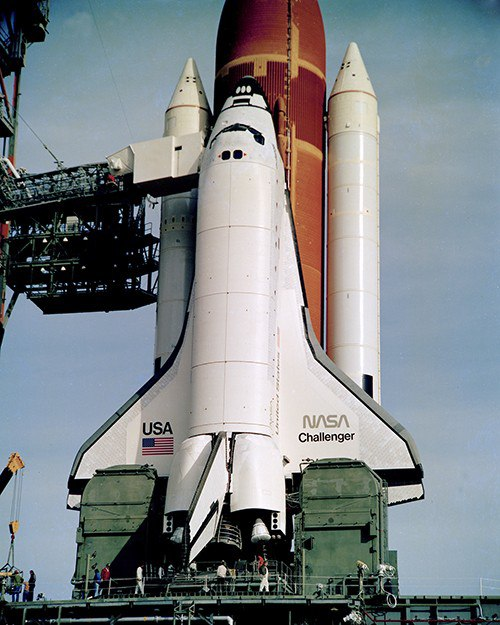
\includegraphics[width=8cm, height=10cm]{figures/challenger.jpg}
\end{center}

En la mañana del 28 de enero de 1986 en Cabo Cañaveral, el transbordador
espacial de la NASA, Challenger estaba sentado en la plataforma de despegue a
punto de despegar. Muchos vieron el evento transmitido con optimismo, mientras
aumentaba la preocupación entre los ingenieros de Thiokol (fabricante) de la
nave espacial debido a las temperaturas significativamente bajas antes del
despegue, lo que puede causar un problema con el transbordador que contiene sus
gases calientes.

La NASA ignoró estas advertencias y decidió continuar con el lanzamiento
programado. Desafortunadamente, las sospechas de los ingenieros resultaron ser
correctas; 73 segundos de vuelo. El transbordador explotó por completo. Además,
esto condujo a la muerte de los siete astronautas.

Debería haber sido un momento histórico. Pero resultó ser uno de los peores
desastres de transbordadores espaciales jamás observados. Se realizaron
investigaciones explorando las causas de la explosión del tanque de combustible
del barco. Lo que finalmente se remonta a las juntas tóricas que evitaban la
fuga de gas caliente.

Ha habido muchas acusaciones y argumentos sobre quién tiene la culpa, pero una
comprensión profunda del desastre requiere un análisis estadístico de los datos
disponibles de las juntas tóricas que contienen información sobre la temperatura
y las tasas de éxito/fallo.

Analizar las fallas de las juntas tóricas requiere una comprensión de la
estructura subyacente de Challenger. Los propulsores de cohetes del
transbordador tenían cuatro segmentos. En primer lugar, lleno de combustible. En
segundo lugar, oxidante. Y la NASA los ensambló y selló con juntas tóricas, un
componente crítico que evitó la fuga de gas caliente durante el lanzamiento.


Sin embargo, la capacidad de respuesta de los sellos no se probó en temperaturas
frías.


El día del lanzamiento, la temperatura era de 31 grados Fahrenheit,
significativamente más baja que las temperaturas en las que se probaron las
juntas tóricas. Después del despegue, una de las juntas tóricas se rompió, lo
que provocó que el gas caliente calentara el oxígeno líquido y el hidrógeno
dentro de los tanques. finalmente rompiendo los propulsores y destrozando el
transbordador 1 . Entonces, ¿por qué se tomó la decisión de continuar con el
lanzamiento, a pesar de las advertencias de los ingenieros?


Antes del lanzamiento del Challenger, nadie había analizado la asociación entre
la temperatura y la capacidad de respuesta de las juntas tóricas. La NASA
decidió arriesgarse al lanzar el transbordador, sin conocer la verdadera
probabilidad estadística de fallas en las juntas tóricas a 31 grados.

Las preocupaciones de los ingenieros se basaban en sospechas y análisis
incompletos. Los ingenieros solo observaron los datos de las juntas tóricas de
baja temperatura que incluían 4 fallas. Al ignorar los datos sobre vuelos a
temperaturas más altas, la probabilidad de falla calculada fue menor de lo que
debería haber sido 2. Este análisis no solo es incorrecto sino también
peligroso y condujo al desastre.

Se deben tener en cuenta los datos de todos los vuelos que se registraron. Ha
habido muchas fallas de juntas tóricas tanto a altas como a bajas temperaturas,
pero no se ha medido la fuerza de la asociación entre estas dos variables. Los
ingenieros no pueden simplemente ignorar los vuelos con temperaturas más
altas.

Se requiere un análisis estadístico profundo de la eficiencia de las juntas
tóricas a varias temperaturas para comprender realmente la falla del Challenger.
Las intuiciones y los análisis sesgados, especialmente por parte de la
administración de la NASA, no son suficientes para determinar la probabilidad de
falla de las juntas tóricas.

A continuación se muestra una muestra de los datos de fallas de las juntas
tóricas:

\begin{center}  
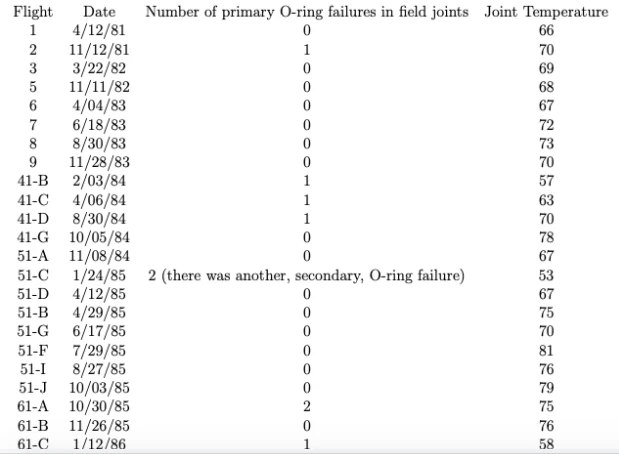
\includegraphics{figures/challenger_data.jpg}
\end{center}

Muestra de datos de juntas tóricas 3.

Se puede ejecutar una prueba de permutación para evaluar la importancia
estadística de la diferencia entre la tasa de falla de la junta tórica a bajas
temperaturas y la tasa de falla a altas temperaturas. Esto puede determinar si
las juntas tóricas de temperatura más baja tienden a experimentar más fallas que
las juntas tóricas de temperatura alta, o si la distribución de fallas es la
misma entre las dos. Las hipótesis de esta prueba estadística son las
siguientes:


\begin{center}  
$H_o: Falla_{bajaTemperatura} - Falla_{altaTemperatura} = 0$
\end{center}


La verdadera diferencia media entre la tasa de falla de la junta tórica a baja y
alta temperatura es 0. Las diferencias observadas se deben al azar.


\begin{center}  
$H_o: Falla_{bajaTemperatura} - Falla_{altaTemperatura} > 0$
\end{center}


La verdadera diferencia media entre la tasa de falla de la junta tórica a baja y
alta temperatura es mayor que 0. Las diferencias observadas no se deben al azar,
sino a una asociación entre la temperatura y la tasa de falla.

La permutación se ejecuta agrupando cada punto de datos en dos grupos. Alta y
baja temperatura. Mirando la distribución de temperatura. Las observaciones de
juntas tóricas se pueden dividir en menos de 65 grados (baja temperatura). Y por
encima de 65 grados (alta temperatura).

La diferencia media observada de fallos entre juntas tóricas de baja y alta
temperatura es de 1,3; la columna de temperatura se permuta (baraja). Y la
diferencia de falla media simulada la calculamos nuevamente entre los dos grupos
de juntas tóricas. La ejecución de 10 000 simulaciones de esta prueba de
permutación produce 10 000 estadísticas de prueba simuladas. A partir de esto,
podemos calcular el valor $p$ para evaluar la hipótesis nula:


\begin{center}  
\begin{align*} 
\frac{sum(diferencias\;simuladas> diferencia\;observada)}{total\; intentos}) = \frac{sum(diferencias \;simuladas>1.3)}{1000}= \\
=0.012
\end{align*}
\end{center}



Solo el $1,2 \%$ de las diferencias medias de fallas simuladas son mayores que
la diferencia media de fallas observada. Un valor p de 0.012 es estadísticamente
significativo para rechazar la hipótesis nula que establece que las tasas de
falla de las juntas tóricas en temperaturas bajas y altas provienen de la misma
distribución.

La diferencia observada es mucho mayor que las diferencias en los datos de las
juntas tóricas barajadas. Esto sugiere que la tasa de fallas entre las juntas
tóricas de baja y alta temperatura no tiene la misma distribución. \\Los datos
muestran evidencia que respalda la hipótesis alternativa que establece que las
juntas tóricas de baja temperatura tienen una mayor tasa media de fallas que las
juntas tóricas de alta temperatura.

Definitivamente parece haber una diferencia entre las juntas tóricas probadas a
bajas temperaturas. Y las juntas tóricas se probaron a altas temperaturas, pero
es útil examinar el modelo subyacente de los datos.

Es importante estimar la probabilidad de falla de la junta tórica a una
temperatura determinada. Esto se puede hacer ajustando un modelo de regresión
logística a los datos anteriores. Con temperatura como entrada y un valor
binario (1: al menos una falla, 0: ninguna falla) como salida. Ajustamos una
regresión logística con los siguientes parámetros:


\begin{center}  
$P(Falla)= \frac{1}{1+exp^{-(\beta_0+\beta_1*temperatura)}}$
\end{center}

Cuando:

\begin{center}  
$\beta_1$
\end{center}

es el coeficiente de temperatura que mide la asociación y


\begin{center}  
$\beta_0$
\end{center}


es el sesgo.

Además, probamos la fuerza de la asociación calculando un valor z con respecto a
las siguientes hipótesis:



\begin{center}  
$H_0 : \beta_1 = 0$
\end{center}


El verdadero coeficiente de temperatura para el modelo es 0, lo que indica que
no hay relación entre la temperatura y la falla de la junta tórica.


\begin{center}  
$H_0 : \beta_1 \not {0}$
\end{center}

El verdadero coeficiente de temperatura para el modelo no es 0, lo que indica
alguna relación entre la temperatura y la falla de la junta tórica.\\

Ajustar los datos a una regresión logística genera un modelo con los siguientes
pesos:

\begin{center}  
$P(Falla)= \frac{1}{1+exp^{-(10.88+0.17*temperatura)}}$
\end{center}


Una gráfica a continuación visualiza la distribución de fallas y el ajuste del modelo:


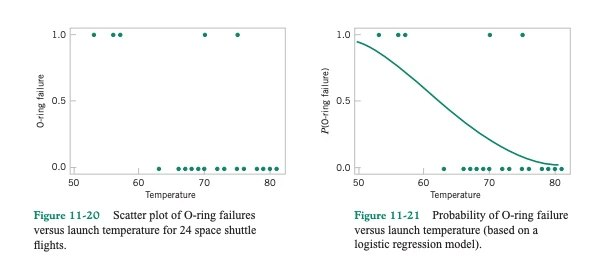
\includegraphics[width=15cm, height=10cm]{figures/challenger_plots.jpg}

Gráfica de regresión logística de datos de juntas tóricas 

Como se observa en la gráfica, una temperatura de 31 grados parece
increíblemente probable que tenga al menos una falla. El modelo genera un valor
de 0,996, lo que indica un $99,6 \%$ de probabilidad de falla dados los datos
observados de lanzamientos de transbordadores anteriores.

Esto está lejos de ser una decisión cerrada y ciertamente no es una apuesta
arriesgada cuando hay siete compañeros de tripulación a bordo.

Además, la fuerza de la asociación entre estas dos variables. Analizamos con el
estadístico z generado en el peso del modelo del coeficiente de temperatura. El
valor $p$ calculado de la hipótesis nula:


\begin{center}  
$H_0 : \beta_1 = 0$
\end{center}


resulta ser 0,04, que es estadísticamente significativo cuando se utiliza un
umbral de 0,05. Debido al bajo valor de p, rechazamos la hipótesis nula que
establece que el coeficiente de temperatura es 0. Existe una fuerte evidencia en
los datos que respalda la hipótesis alternativa:

\begin{center}  
$H_0 : \beta_1 > 0$
\end{center}


lo que sugiere que el coeficiente es mayor que 0 y que, de hecho, existe una
asociación entre la temperatura y la falla de la junta tórica. Por lo tanto,
existe una fuerte evidencia de que las bajas temperaturas pueden provocar fallas
en las juntas tóricas. Además, los ingenieros deberían haber presentado un
análisis de regresión logística como evidencia para retrasar el lanzamiento del
Challenger.\\

Hay muchas explicaciones posibles de por qué los funcionarios de la NASA
decidieron ignorar todas las advertencias de los ingenieros de Thiokol y
continuar con el lanzamiento. Algunos dicen que se debió al simple hecho de que
la NASA quería demostrar que otros estaban equivocados y mantener su ambicioso
programa de lanzamiento.\\

Otros argumentan que se debió a razones burocráticas. La Casa Blanca presionó a
la NASA para realizar el lanzamiento. Entonces Reagan podría mencionarlo en su
discurso sobre el estado de la unión. Además, la dirección se produjo el mismo
día. No importa la razón, la NASA no debería haber hecho una apuesta tan grande
y debería haber retrasado el lanzamiento para otro día.\\
El análisis de los datos retrata claramente los riesgos, pero nadie había hecho
una investigación exhaustiva de antemano. Como resultado del desastre, el
Congreso cerró el programa de transbordadores espaciales durante años. Hasta que
la NASA abordó sus problemas internos.\\

La NASA hizo una extensa investigación sobre sus propios fracasos. Y la NASA
implementó cambios significativos para abordar las incompetencias existentes.
Además, la NASA publicó informes de investigación que describen la incapacidad
de la junta tórica para mantener su elasticidad después de la exposición a bajas
temperaturas.\\

La Casa Blanca formó un comité presidencial para investigar asuntos internos en
la NASA. Y supervisar la reestructuración de la planificación y gestión de
misiones. La NASA remodeló una parte significativa del diseño actual del
transbordador para reducir los riesgos de puntos de falla.\\

Capacitación de gestión fuertemente aplicada por la NASA. Esto cambió la
dinámica de la cultura laboral. Los funcionarios y los ingenieros fueron todos
responsables de abordar todas las inquietudes que surgieron durante el proceso
de lanzamiento 5 . La NASA tardó dos años en reparar los daños, reestructurar y
reabrir.\\
Este desastre se convirtió en la base para que la NASA mejorara su toma de
decisiones y la coordinación entre ingenieros y administradores. Después de
cambiar las operaciones internas y establecer nuevos estándares éticos y de
producción, la NASA continuó con su programa de transbordadores espaciales con
misiones mejor administradas. Discovery fue la primera misión después de la
reapertura y transcurrió sin problemas. Esto se convirtió en el advenimiento de
una serie de misiones exitosas aprendiendo de los errores cometidos en
Challenger.\\

El desastre del Challenger muestra por qué los científicos e ingenieros
necesitan comprender las técnicas estadísticas. Los análisis básicos descritos
brindan una sólida evidencia cuantitativa de que el transbordador no debería
haberse lanzado debido a la probabilidad significativamente alta de falla de la
junta tórica, un componente crítico de la nave espacial.\\

La NASA ahora ha hecho del análisis estadístico y de riesgo de cada componente
del transbordador una prioridad antes del lanzamiento. Es probable que este
estándar prevenga muchos desastres futuros y promueva la expansión del programa
de exploración espacial de los Estados Unidos.\\





\section{Distribución de Poisson}

Supongamos que estamos interesados en conteos que ocurren en un intervalo de
tiempo (por ejemplo, dentro de una hora en particular). Debido a que son
conteos, no son negativos y tienen un valor entero. Sabemos que estos recuentos
tienen dos propiedades importantes. Primero, ocurren con alguna tasa promedio
fija. En segundo lugar, se produce una observación independientemente del
intervalo desde la última observación. Entonces la distribución de Poisson es un
modelo apropiado \cite{forsyth2018probability}.

\begin{theorem}{Distribución de Poisson}{Poisson}
Una variable aleatoria $X$, no negativa de valor entero, tiene una distribución de
Poisson cuando su distribución de probabilidad toma la forma:

\begin{equation}
    P({X=k})=\lambda^k e^{-\lambda}
\end{equation}

Donde $\lambda > 0$ es un parámetro conocido como la intensidad de la distribución.
    
\end{theorem}

La distribución de Poisson es una distribución de probabilidad, porque es no
negativa y porque:

\begin{center}
    \[
\sum_{i=0}^{\infty} \frac{\lambda^i}{i!} = e^\lambda
\]
\end{center}

tal que,

\begin{center}
    \[
\sum_{k=0}^{\infty} \frac{\lambda^i e^\lambda}{i!}  = 1
\]
\end{center}

Una distribución de Poisson con intensidad $\lambda$ tiene:

\begin{itemize}
    \item Media $\lambda$;
    \item Varianza $\lambda$
\end{itemize}

La distribución de Poisson se usa a menudo en situaciones en las que contamos el
número de éxitos en una región o intervalo de tiempo en particular, y hay una
gran cantidad de intentos, cada uno con una pequeña probabilidad de éxito
\cite{blitzstein2015introduction}.

Por ejemplo, las siguientes variables aleatorias podrían seguir una distribución
que es aproximadamente Poisson.

\begin{itemize}
\item El número de correos electrónicos que recibe en una hora. Hay muchas
personas que potencialmente podrían enviar un correo electrónico en esa hora,
pero es poco probable que una persona específica realmente le envíe un correo
electrónico en esa hora. Alternativamente, imagina subdividir la hora en
milisegundos. Hay $3.6 \times 10^6$ segundos en una hora, pero en cualquier
milisegundo específico es poco probable que reciba un correo electrónico.

\item El número de chispas en una galleta con chispas de chocolate. Imagina
subdividir la galleta en cubos pequeños; la probabilidad de obtener una chispa
de chocolate en un solo cubo es pequeña, pero el número de cubos es grande.

\item El número de terremotos en un año en alguna región del mundo. En cualquier
momento y lugar dados, la probabilidad de un terremoto es pequeña, pero hay una
gran cantidad de posibles momentos y lugares para que ocurran terremotos en el
transcurso del año.

\end{itemize}

\subsection{Aproximación a la distribución de Poisson a partir de la Binomial.}

La distribución binomial depende de 3 parámetros:

  \begin{equation}
    f(x,n,p) = \binom{n}{x} p^x (1-p)^{n-x}
  \end{equation}

Entonces, queremos saber si existe una relación entre el experimento actual y el
anterior.

Por lo que podemos hacer:

\begin{equation}
  \begin{array}{rr}
  \frac{f(x,n,p)}{f(x-1,n,p)} = & \frac{\binom{n}{x} p^x (1-p)^{n-x}}{\binom{n}{x-1} p^{x-1} (1-p)^{n-(x-1)}} \\
  \\
%                              = & \frac{\binom{n}{x} p^x (1-p)^{n} (1-p)^{-x}}{\binom{n}{x-1} \frac{p^x}{p} (1-p)^{n}(1-p)^{-(x-1)}} \\

                              = & \frac{\binom{n}{x} p^x (1-p)^{n} (1-p)^{-x}}{\binom{n}{x-1} \frac{p^x}{p} (1-p)^{n}(1-p)^{-x} (1-p)}
  \end{array}
\end{equation}

\begin{equation}
  \begin{array}{rr}
  \frac{f(x,n,p)}{f(x-1,n,p)} = & \frac{\binom{n}{x} p}{\binom{n}{x-1} (1-p)} \\
  \\
                              = & \frac{\binom{n}{x} p}{\binom{n}{x-1} q} \\
  \end{array}
\end{equation}

Pero...
  
\begin{equation}
  \begin{array}{rr}
  \frac{\binom{n}{x}}{\binom{n}{x-1}} = & \frac{\frac{n!}{(n-x)!x!}}{\frac{n!}{(n-(x-1))!(x-1)!}} \\
  \\
                                      = & \frac{n-x+1}{x}
  \end{array}
\end{equation}

Por lo que...

\begin{equation}
  \begin{array}{rr}
  \frac{f(x,n,p)}{f(x-1,n,p)} = & \frac{n-x+1}{x} \cdot \frac{p}{q}
  \end{array}
\end{equation}

\begin{equation}
  \begin{array}{rr}
  \frac{f(x,n,p)}{f(x-1,n,p)} = & \frac{(n+1)p - xp}{xq} \\
  \\
                              = & \frac{(n+1)p - x(1-q)}{xq} \\
  \\
                              = & \frac{(n+1)p - x + xq}{xq} \\
  \\
                              = & 1 + \frac{(n+1)p - x}{xq} \\
  \end{array}
  \label{eq:poissonGral}
\end{equation}

Ahora podemos hacer el caso cuando $x=0$:

\begin{equation}
  f(0,n,p) = \binom{n}{0} p^0 (1-p)^{n-0} = (\frac{n!}{(n-0)! 0!})(1-p)^n = (1-p)^n
\end{equation}

Pero sabemos que la esperanza matemática $\lambda = np \Rightarrow p =
\frac{\lambda}{n}$,
  
entonces,

\begin{equation}
  f(0,n,p) = (1-\frac{\lambda}{n})^n
\end{equation}

Podemos hacer que:

\begin{equation}
  \ln(f(0,n,p)) = n \ln((1-\frac{\lambda}{n}))
\end{equation}

Usando la serie de Taylor:

\begin{equation}
  \ln(1+x) = x - \frac{x^2}{2} + \frac{x^3}{3} - \frac{x^4}{4} + ...
\end{equation}

Tenemos que:

\begin{equation}
  \begin{array}{rl}
  \ln(1+(-\frac{\lambda}{n})) = & (-\frac{\lambda}{n}) - \frac{(-\frac{\lambda}{n})^2}{2} + \frac{(-\frac{\lambda}{n})^3}{3} - \frac{(-\frac{\lambda}{n})^4}{4} + ... \\
  \\
                              = & -\frac{\lambda}{n} + \frac{\lambda^2}{2n^2} - \frac{\lambda^3}{3n^3} - \frac{\lambda^4}{4n^4}+...
  \end{array}
\end{equation}

Pero sabemos que $n \to \infty$, por lo que nos queda:

\begin{equation}
  n \ln(1-\frac{\lambda}{n}) = -\lambda
\end{equation}  

Sabiendo que: \\

$ \lim_{n \to \infty} [\ln (f(0,n,p))] = \lim_{n \to \infty} (1 -
\frac{\lambda}{n})^n = -\lambda$


Quitando el $\ln$, podemos concluir que para $n=0$,

\begin{equation}
  f(0,n,p) = e^{-\lambda}
\end{equation}

Si $x=1$, a partir de la Ec. \eqref{eq:poissonGral}, tenemos:

\begin{equation}
  \begin{array}{rl}
  f(1,n,p)  = & (1 + \frac{(n+1)p - 1}{q}) \cdot f(0,n,p) \\
  \\
            = & (\frac{q + (n+1)p - 1}{q}) \cdot e^{-\lambda} \\
  \\
            = & (\frac{q + p + np - 1}{q}) \cdot e^{-\lambda} \\
  \\
            = & (\frac{np}{q}) \cdot e^{-\lambda} \\
  \\
            = & (\frac{\lambda}{q}) \cdot e^{-\lambda} \\
  \end{array}
\end{equation}

Siempre que $n \to \infty$ y $p \to 0 \Rightarrow q \to 1$, porque $q=1-p$
Entonces:

\begin{equation}
f(1,n,p) = \lambda e^{-\lambda}
\end{equation}

Si $x=2$, a partir de la Ec. \eqref{eq:poissonGral}, tenemos:

\begin{equation}
  \begin{array}{rl}
  f(2,n,p)  = & (1 + \frac{(n+1)p - 2}{2q}) \cdot f(1,n,p) \\
  \\
            = & (\frac{2q + (n+1)p - 2}{2q}) \cdot \lambda e^{-\lambda} \\
  \\
            = & (\frac{2q + np + p - 2}{2q}) \cdot \lambda e^{-\lambda} \\
  \\
            = & (\frac{2(1-p) + np + p - 2}{2q}) \cdot \lambda e^{-\lambda} \\
  \\
            = & (\frac{2 - 2p + np + p - 2}{2q}) \cdot \lambda e^{-\lambda} \\
  \\
            = & (\frac{np - p}{2q}) \cdot \lambda e^{-\lambda} \\
  \end{array}
\end{equation}

Pero $np=\lambda$

\begin{equation}
  f(2,n,p)  = (\frac{\lambda - p}{2q}) \cdot \lambda e^{-\lambda}
\end{equation}

Pero si $p \to 0$, entonces $q \to 1$ porque $q=1-p$
Entonces, tenemos que:

\begin{equation}
  f(2,n,p)  = (\frac{\lambda}{2}) \cdot \lambda e^{-\lambda}
\end{equation}

Sabemos que si $x=0$: \\
$f(0,n,p) = \frac{\lambda^0}{0!} e^{-\lambda}$\\

Si $x=1$: \\
$f(1,n,p) = \frac{\lambda^1}{1!} e^{-\lambda}$\\

Si $x=2$: \\
$f(2,n,p)  = \frac{\lambda^2}{2!} \cdot \lambda e^{-\lambda}$\\


Entonces, si $x=k$:

\begin{equation}
  f(k,n,p)  = \frac{\lambda^k}{k!} \cdot \lambda e^{-\lambda}
\end{equation}

Esta es la función de probabilidad de Poisson de V.A. Así, podemos definir tres
parámetros importantes:

\begin{enumerate}
  \item Valor esperado:
  \begin{equation}
    \mu = E(x) = \sum_{x} xf(x) = \sum_{x} \frac{x e^{-\lambda}\lambda^k}{x!} = \lambda
  \end{equation}

\item Varianza:
\begin{equation}
  \sigma^2 = \sum_{x} \frac{x^2 e^{-\lambda}\lambda^k}{x!} - (\sum_{x} \frac{x e^{-\lambda}\lambda^k}{x!})^2 = \lambda
\end{equation}

\item Desviación estándar:
\begin{equation}
  \sigma = \sqrt{\lambda}
\end{equation}

\end{enumerate}

\subsection{Ejemplo de la distribución de Poisson}

El número de incidentes de tránsito que ocurren en una cierta avenida en un día
cualquiera sigue una distribución Poisson de media $\lambda=1$. Entonces:

  \begin{figure}
    \centering
    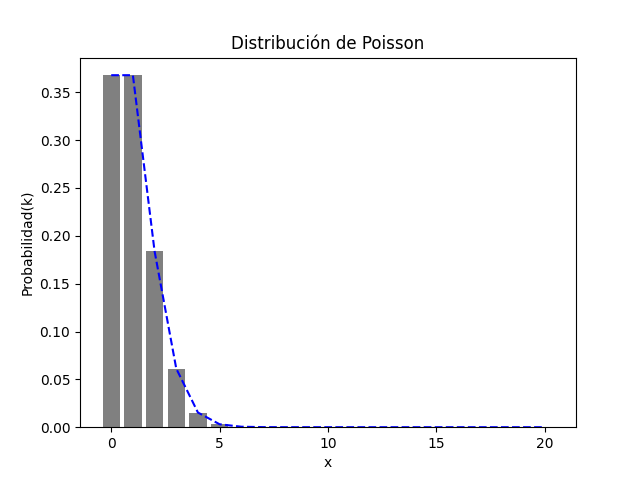
\includegraphics[scale=0.9]{../slides/figures/poisson_distribution_lambda_1.png}
  \end{figure}

El número de incidentes de tránsito que ocurren en una cierta avenida en un día
cualquiera sigue una distribución Poisson de media $\lambda=4$. Entonces:

  \begin{figure}
    \centering
    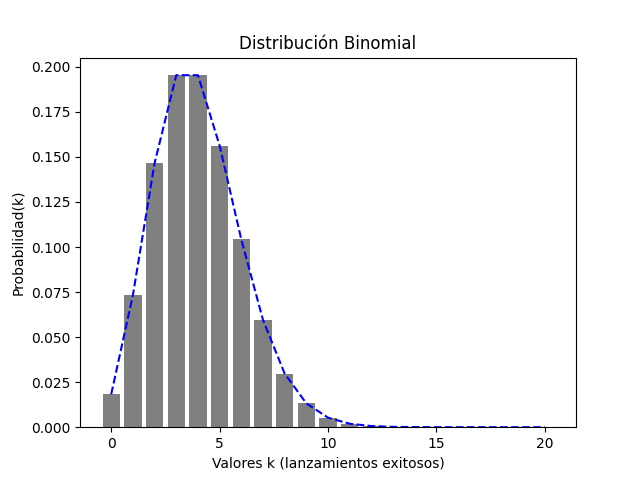
\includegraphics[scale=0.9]{../slides/figures/poisson_distribution_lambda_4.png}
  \end{figure}

El número de incidentes de tránsito que ocurren en una cierta avenida en un día
cualquiera sigue una distribución Poisson de media $\lambda=10$. Entonces:

\begin{figure}
    \centering
  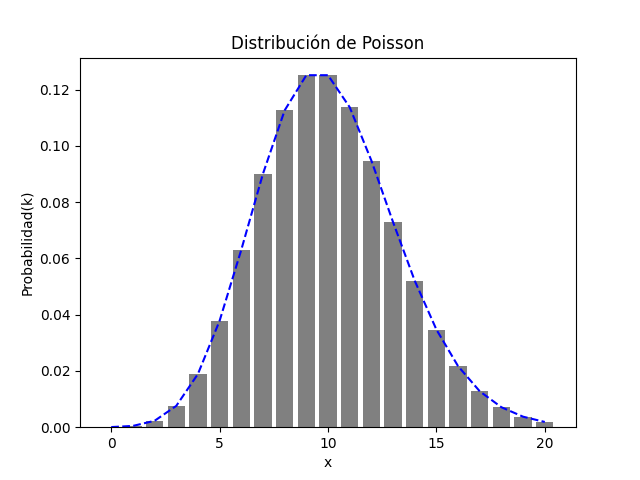
\includegraphics[scale=0.9]{../slides/figures/poisson_distribution_lambda_10.png}
\end{figure}



%\section{Distribuci\'on exponencial}

Decimos que una variable aleatoria continua $X$ tiene distribución exponencial
con parámetro $\lambda > 0$, y escribimos $X \sim \text{exp}(\lambda)$, cuando
su función de densidad es:

\begin{equation}
    f(x) = \left\lbrace \begin{array}{ll}
        \lambda e^{-\lambda x} & \text{ si } x>0, \\
        0 & \text{ en otro caso.}
    \end{array}\right.
\end{equation}

La gráfica de esta función, cuando el parámetro $\lambda$ toma el valor
particular 3. La correspondiente función de distribución aparece a su derecha.
Es muy sencillo verificar que la función $f(x)$ arriba definida, es
efectivamente una función de densidad para cualquier valor del parámetro
$\lambda > 0$. Se trata pues de una variable aleatoria continua con valores en
el intervalo $0, \infty$. Esta distribución se usa para modelar tiempos de
espera para la ocurrencia de un cierto evento.



\pagebreak
\bibliography{../references/references.bib} 
\bibliographystyle{unsrt}

\end{document}

%poner alef 1 y alef2
% Axiomas de peano
